\documentclass[11pt]{article}

% ACL style
\usepackage[review]{acl}

% Standard font packages
\usepackage{times}
\usepackage{latexsym}
\usepackage{inconsolata}

% Character encoding
\usepackage[T1]{fontenc}
\usepackage[utf8]{inputenc}

% Improved layout
\usepackage{microtype}

% Math
\usepackage{amsmath}
\usepackage{amssymb}

% Tables and figures
\usepackage{booktabs}
\usepackage{graphicx}
\graphicspath{{figures/}}
\usepackage{subcaption}
\usepackage{multirow}
\usepackage{array}
\usepackage{tabularx}
\usepackage{adjustbox}
\usepackage{placeins}

% Cross-references
\usepackage[capitalize]{cleveref}

% Enumerate
\usepackage{enumitem}

\title{Acquiescence Is Not Personality:\\ Why Human Psychometric Instruments Fail on LLMs}

\author{Anonymous Authors}

\date{}

\begin{document}
\maketitle

\begin{abstract}
Large language models are increasingly used as agents with different personalities in surveys, social simulation, and public-opinion studies. A common practice is to give an LLM a personality label, ask it to answer human personality questionnaires, and treat the resulting scores as the agent's personality. But this assumes that these questionnaires measure personality in LLMs the same way they do in humans.We test this assumption with a 221-item personality battery across 20 LLMs and 17 persona settings, collecting 375,700 responses. The results show that this assumption does not hold. LLMs tend to agree with questionnaire statements regardless of whether the statements point in opposite directions. This acquiescence bias makes reverse-coded items inconsistent, distorts reliability scores, and collapses the expected personality factor structure.Persona prompts can make LLMs answer in ways that look like different personalities. But this does not mean that the questionnaire is measuring real personality traits. If a trait is real, the model should answer opposite items in opposite ways. Instead, LLMs often agree with both a statement and its reverse, suggesting that the score is driven by a general tendency to agree rather than by the intended trait. Therefore, persona prompting shows that LLMs can imitate personality roles, but questionnaire scores alone are not reliable evidence of stable personality traits for LLM agents or social simulations.
\end{abstract}

\section{Introduction}

Large language models (LLMs) are increasingly treated as agents with personalities. Prior work administers human personality questionnaires to LLMs, computes trait scores, and reports personality profiles \citep{miotto2023gpt3, bhandari2025evaluating, serapio2025psychometric, sorokovikova2024evaluating, lee2025trait, jiang2023personallm, huang2023psychobench}. These scores are also used to support ``silicon samples'' for surveys and behavioural experiments \citep{argyle2023one, horton2023homo, aher2023using, park2023generative, ferreira2025matching}, as well as persona-conditioned simulations of opinion dynamics, debate, and polarisation \citep{chuang2023simulating, cau2025language, chuang2025debate}. However, these applications rely on a basic assumption: that human personality questionnaires actually measure meaningful traits in LLMs. This paper tests that assumption.

\begin{figure}[t]
\centering
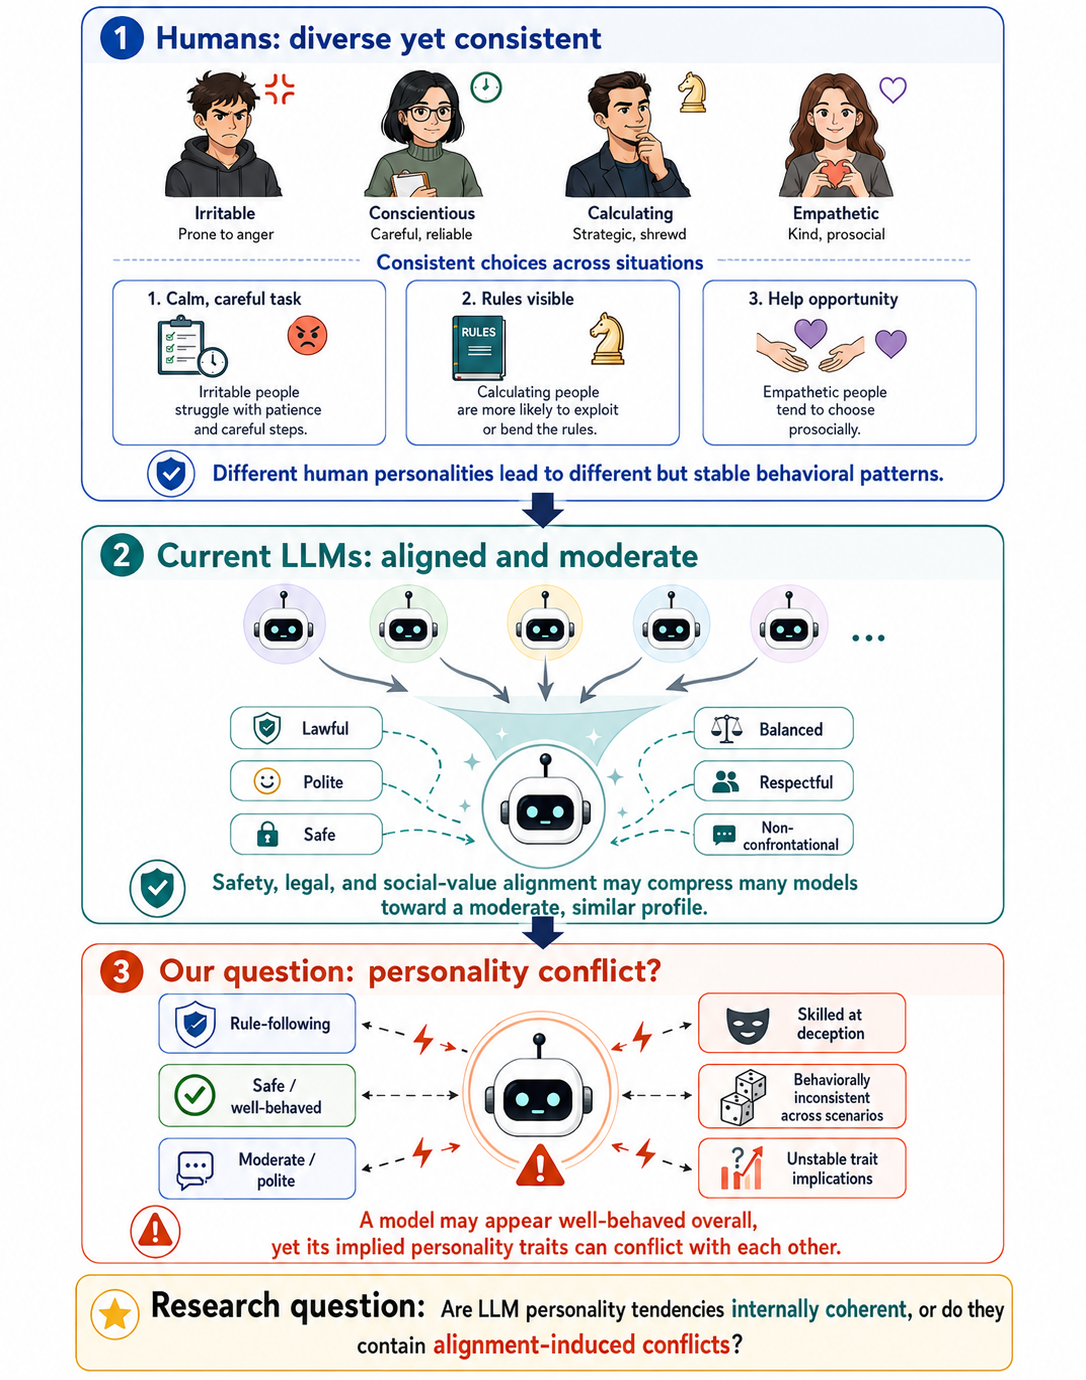
\includegraphics[width=0.9\linewidth]{fig1_research_question_concept.png}
\caption{The question this paper asks. Rather than reporting LLM personality scores, we test whether the instruments produce valid measurement at all.}
\label{fig:research-question}
\end{figure}
\FloatBarrier

The distinction is important. An LLM may follow a prompt such as ``act as an extraverted person'' and give answers that look extraverted. But this does not mean that a personality questionnaire has measured a stable trait. A valid trait measure should give consistent answers to items with the same meaning and opposite answers to items with opposite meanings. It should also recover the expected factor structure, agree with related scales, and remain comparable across models and prompt conditions \citep{cronbach1951coefficient, lord1968statistical}. These checks are standard in human psychometrics, but are rarely applied to LLM personality scores.

We evaluate this measurement foundation directly. We administer a 221-item battery, including IPIP-NEO-120, SD3, ZKPQ-50-CC, and EPQR-A, to 20 LLMs under 17 persona settings, collecting 375,700 responses. Across standard psychometric checks, the instruments fail to produce valid measurement. The failures trace to a common response style: acquiescence. LLMs often agree with statements regardless of whether the statements point in opposite directions. This makes forward- and reverse-coded items inconsistent, distorts reliability, collapses the expected five-factor structure into three factors, and leaves model identity explaining less than 1\% of the variance.

Persona prompts do change LLM responses, but they do not fix this problem. They show that models can follow personality instructions, not that questionnaire scores validly measure personality traits. Our results therefore caution against treating questionnaire-derived scores as evidence that LLM agents have stable, human-like personalities, especially when such scores are used to ground social simulation.

% \section{Related Work}

% \subsection{Personality Measurement in LLMs}

% Researchers have administered personality questionnaires to LLMs and reported personality profiles \citep{miotto2023gpt3, serapio2025psychometric, bhandari2025evaluating, sorokovikova2024evaluating, lee2025trait, hagendorff2024machine, jiang2023personallm, huang2023psychobench}. But almost none of these studies check whether the instruments actually work on LLMs the way they work on humans. Benchmarks show systematic deviations between LLM and human responses \citep{xie2025aipsychobench}, temporal stability is limited \citep{bodroza2024personality}, and measurement invariance is assumed rather than tested \citep{suhr2025challenging}. \citet{chen2025humanizing} noted that most existing frameworks skip psychometric validation entirely. \citet{schaekermann2024personality} report partial reliability checks, and \citet{han2025personality} expose a dissociation between LLM self-reports and downstream behaviour.

% These profiles in turn feed into two downstream programmes. The silicon-sample literature \citep{argyle2023one, horton2023homo, aher2023using, ferreira2025matching} uses LLM personality scores to simulate human survey respondents; the persona-conditioned multi-agent literature \citep{chuang2023simulating, cau2025language, chuang2025debate, park2023generative} embeds persona-conditioned LLMs in interactive social simulations of opinion dynamics, debate, and trust. Both programmes inherit whatever measurement error sits in the underlying personality scores. \citet{larooij2025validation} systematically review this literature and identify validation as the central unmet challenge: existing simulations rely on face validity rather than calibration grounded in psychometric measurement. \citet{mannekote2025roleplaying} extend the self-report--behaviour dissociation to role-playing trust agents.

% Previous work asks ``what personality does this LLM have?'' and reports scores. We ask a different question: do these instruments measure anything meaningful at all when given to LLMs? Instead of profiling, we run the full set of standard psychometric validation checks (internal consistency, factor structure, convergent validity, reverse-item consistency, measurement invariance, and variance decomposition) on a single dataset covering 20 models and 221 items.

% \subsection{Response Style and Acquiescence Bias}

% Survey respondents do not always answer based on content alone. Acquiescence bias (agreeing with statements regardless of direction) is one of the most studied response styles, introduced as ``yea-saying'' by \citet{couch1960yeasayers} and formalised alongside social desirability by \citet{crowne1960social} and \citet{paulhus1991response}. \citet{billiet2000modeling} model acquiescence as an explicit factor in structural-equation models of balanced item sets, and \citet{baumgartner2007modeling} document its cross-national footprint. The standard countermeasure is reverse-keyed items: items written so that endorsement maps to the negative pole of the trait. \citet{acerbi2024llm} and \citet{salecha2024llm} showed that LLMs also exhibit social desirability biases in Big Five surveys, and \citet{acquiescence2025emnlp} confirmed that acquiescence in LLMs is robust across languages. Forced-choice and ipsative inventories built on item-response theory have been proposed as structural alternatives that bypass response styles entirely \citep{brown2011forcedchoice, treaux2025forced}.

% These studies documented that acquiescence and social desirability exist in LLM responses. Our approach is different: we quantify the measurement damage they cause by decomposing the bias at item level, separating forward-coded and reverse-coded agree rates, and comparing across instruments with different content (normal personality vs.\ dark traits).

% \subsection{Alignment Effects on LLM Behavior}

% RLHF and safety training make LLMs more helpful and harmless, but also more homogeneous \citep{ouyang2022training, bai2022constitutional, wei2022flan}. \citet{sharma2024sycophancy} showed that aligned models tend to echo user opinions even when wrong, and \citet{zheng2024agreeableness} linked Agreeableness scores to sycophancy in role-playing LLMs. \citet{wang2024aligning} argued that RLHF encodes a specific notion of acceptability that may override genuine variation. \citet{kirk2023understanding} show that RLHF systematically reduces output diversity and homogenises generation distributions, and \citet{perez2023discovering} use model-written evaluations to surface a wide spectrum of value-laden behaviours including sycophancy. \citet{rafailov2023dpo} introduce direct preference optimisation as an alternative to RLHF, and \citet{christiano2017deep} established the original deep RL-from-human-preferences framework.

% These studies examined alignment effects on individual behaviors. We take a different angle: we test whether alignment produces a universal response style across model families via DIF analysis, and we quantify how far persona injection can push a model from its default behavior (Persona Separation Degree).

\section{Related Work}

\subsection{Personality Measurement in LLMs}

Many studies administer human personality questionnaires to LLMs and report personality profiles \citep{miotto2023gpt3, serapio2025psychometric, bhandari2025evaluating, sorokovikova2024evaluating, lee2025trait, hagendorff2024machine, jiang2023personallm, huang2023psychobench}. However, these instruments are often used without testing whether they remain valid for LLMs. Existing work already suggests problems: LLM responses differ from humans \citep{xie2025aipsychobench}, show limited temporal stability \citep{bodroza2024personality}, assume rather than establish measurement invariance \citep{suhr2025challenging}, and often skip psychometric validation \citep{chen2025humanizing}. Partial reliability and behavioural analyses further question whether self-reported profiles reflect actual behaviour \citep{schaekermann2024personality, han2025personality}. These scores also support ``silicon sample'' studies \citep{argyle2023one, horton2023homo, aher2023using, ferreira2025matching} and persona-based social simulations \citep{chuang2023simulating, cau2025language, chuang2025debate, park2023generative}, where weak measurement can undermine downstream conclusions \citep{larooij2025validation, mannekote2025roleplaying}. Unlike work that asks what personality an LLM appears to have, we ask whether the questionnaires measure meaningful traits at all.

\subsection{Response Style and Acquiescence Bias}

Acquiescence bias, or agreeing regardless of item direction, is a classic survey response style \citep{couch1960yeasayers, crowne1960social, paulhus1991response}. Psychometric studies model it as a separate factor and show that it can distort scale structure across populations \citep{billiet2000modeling, baumgartner2007modeling}. In LLMs, prior work reports social desirability and acquiescent responding \citep{acerbi2024llm, salecha2024llm, acquiescence2025emnlp}, while forced-choice and ipsative designs have been proposed to reduce response-style effects \citep{brown2011forcedchoice, treaux2025forced}. We extend this line by measuring how acquiescence damages validity: reverse-item consistency, reliability, factor structure, and cross-instrument convergence.

\subsection{Alignment Effects on LLM Behavior}

Alignment methods such as RLHF, constitutional AI, instruction tuning, and preference optimisation shape LLM behaviour \citep{ouyang2022training, bai2022constitutional, wei2022flan, christiano2017deep, rafailov2023dpo}. Prior work links alignment to sycophancy, agreeableness, homogenisation, and value-laden behaviour \citep{sharma2024sycophancy, zheng2024agreeableness, wang2024aligning, kirk2023understanding, perez2023discovering}. We study alignment from a measurement perspective: whether aligned models share a common response style, and how far persona prompting can move them from that default.

\section{Methodology}

\begin{figure*}[t]
\centering
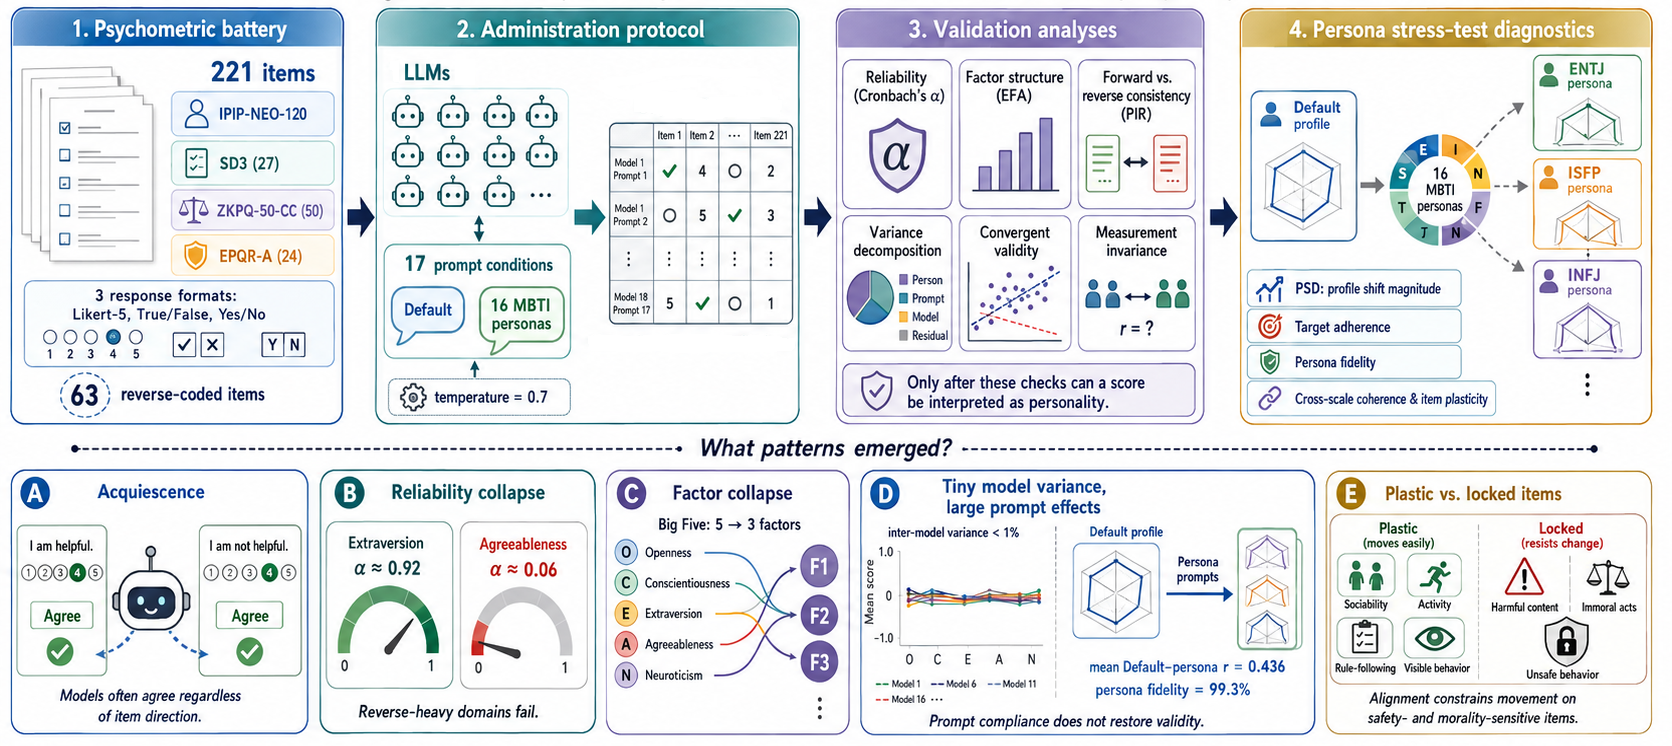
\includegraphics[width=\textwidth]{fig2_methodology_pipeline.png}
\caption{Overview of the methodology. We administer a multi-instrument psychometric battery to LLMs, normalize the response matrix, and run standard validation checks before interpreting any score as evidence of personality.}
\label{fig:methodology-overview}
\end{figure*}

\subsection{Psychometric Instruments}

\Cref{fig:validation_battery_schema} provides an overview of the full diagnostic pipeline. We administered a 221-item battery comprising four validated instruments (\cref{tab:instruments}): IPIP-NEO-120 \citep{johnson2014measuring}, SD3 \citep{jones2014introducing}, ZKPQ-50-CC \citep{aluja2006cross}, and EPQR-A \citep{francis1992development}. Together they cover 17 domains across three response formats (Likert-5, True/False, Yes/No) and include 63 reverse-coded items.

\begin{table}[t]
\centering
\small
\caption{Psychometric instruments in the 221-item battery.}
\label{tab:instruments}
\begin{tabular}{lrrrr}
\toprule
Instrument & Items & Format & Domains & Rev. \\
\midrule
IPIP-NEO-120 & 120 & Likert-5 & 5 & 41 \\
SD3 & 27 & Likert-5 & 3 & 5 \\
ZKPQ-50-CC & 50 & T/F & 5 & 12 \\
EPQR-A & 24 & Y/N & 4 & 5 \\
\midrule
\textbf{Total} & \textbf{221} & 3 formats & \textbf{17} & \textbf{63} \\
\bottomrule
\end{tabular}
\end{table}

\subsection{Models and Administration Protocol}

We tested 20 LLMs spanning 8 model families (\cref{tab:models}), covering both proprietary and open-weight systems. Technical details for each family are available in the respective model reports \citep{openai2023gpt4, gemini2024v15, deepseek2024v3, qwen2024qwen25, glm2024chatglm, moonshot2025kimi, minimax2025minimax01}.

\begin{table}[t]
\centering
\small
\caption{All 20 tested LLMs grouped by model family.}
\label{tab:models}
\begin{tabular}{l>{\centering\arraybackslash}p{5.2cm}}
\toprule
Family & Models \\
\midrule
Anthropic & Claude Opus 4.6, Sonnet 4.6 \\
OpenAI & GPT-5.5, GPT-5.2 \\
DeepSeek & V3.2, V4-Flash, V4-Pro \\
Google & Gemini-3-Flash, Gemini-3.1-Flash-Lite, Gemini-3.1-Pro, Gemini-3-Pro \\
Alibaba & Qwen3-235B-A22B, Qwen3.5-122B-A10B, Qwen3.5-397B-A17B \\
Moonshot & Kimi-K2.5, Kimi-K2.6 \\
MiniMax & M2.7 \\
Zhipu & GLM-4.6V, GLM-4.7, GLM-5.1 \\
\bottomrule
\end{tabular}
\end{table}

Each model was tested under 17 conditions: a \textbf{Default} prompt (``Please answer the following personality questionnaire honestly.'') and 16 \textbf{MBTI persona} prompts, each assigning a specific MBTI type. All administrations used temperature = 0.7. Each (model, persona, item) cell was sampled 5 times ($k{=}5$). Responses are averaged across samples within each cell. This yielded $20 \times 17 \times 221 = 75{,}140$ item-level scores (averaged from 375{,}700 raw API calls).

\subsection{Analysis Pipeline}

We applied six checks that psychometricians use before trusting any instrument on a new population.

\paragraph{Internal consistency.}
We compute Cronbach's $\alpha$ per IPIP domain for each model, using the 17 persona conditions as observations. For a domain with $k$ items, let $X_{pi}$ be the scored response to item $i$ under persona $p$. Then:
\begin{equation}
\alpha = \frac{k}{k-1}\left(1 - \frac{\sum_{i=1}^{k} \mathrm{Var}(X_i)}{\mathrm{Var}\!\left(\sum_{i=1}^{k} X_i\right)}\right)
\label{eq:cronbach}
\end{equation}
We average $\alpha$ across the 20 models. Human benchmarks come from \citet{johnson2014measuring}.

\paragraph{Factor structure.}
Let $\mathbf{x}_j \in \mathbb{R}^{17}$ be the vector of domain scores for observation $j$ ($j = 1, \ldots, 340$). We standardize each domain to zero mean and unit variance, then compute the correlation matrix $\mathbf{R}$. We retain factors via the Kaiser criterion ($\lambda_i > 1$) \citep{kaiser1960application} and validate with parallel analysis \citep{horn1965parallel}: we permute each column of the data matrix independently, recompute eigenvalues, and repeat 500 times. A factor is retained only if its observed eigenvalue exceeds the 95th percentile of the permuted distribution. We extract factor loadings via eigendecomposition of $\mathbf{R}$ followed by varimax rotation \citep{kaiser1958varimax}. Factor replication across models is assessed with Tucker's coefficient of congruence \citep{tucker1951method}.

\paragraph{Reverse-item consistency.}
For each domain that contains both forward-coded ($+$) and reverse-coded ($-$) items, we compute the Pairwise Inconsistency Rate (PIR). For Likert items, a forward-reverse pair $(f, r)$ is inconsistent when both responses are at or above the midpoint, or both are at or below it:
{\small
\begin{equation}
\mathrm{PIR} = \frac{1}{|F|\,|R|} \sum_{f \in F}\sum_{r \in R} \mathbf{1}\!\bigl[(f \ge 3 \wedge r \ge 3) \vee (f \le 3 \wedge r \le 3)\bigr]
\label{eq:pir}
\end{equation}
}
where $F$ and $R$ are the sets of forward and reverse item responses (raw Likert values), and the midpoint is 3 on the 1--5 scale. For binary items, inconsistency is $f = r$.

\paragraph{Variance decomposition.}
We normalize all scored responses to a common 0--1 scale: Likert scores via $x' = (x - 1)/4$, binary scores kept as-is. We then decompose the total sum of squares into marginal components:
\begin{equation}
\begin{split}
\mathrm{SS}_{\mathrm{total}} &= \sum_{i}(y_i - \bar{y})^2 \\
&= \mathrm{SS}_{\mathrm{model}} + \mathrm{SS}_{\mathrm{domain}} \\
&\quad + \mathrm{SS}_{\mathrm{persona}} + \mathrm{SS}_{\mathrm{item}} + \mathrm{SS}_{\mathrm{resid}}
\end{split}
\label{eq:variance}
\end{equation}
where each component groups by the corresponding factor and computes the squared deviation of group means from the grand mean. We run this separately for Likert and binary scales.

\paragraph{Convergent validity.}
For each of 8 pre-specified construct pairs (e.g., IPIP Neuroticism vs.\ ZKPQ Neuroticism-Anxiety), we compute Pearson $r_p$ and Spearman $r_s$ across the 20 model-level means. A pair passes if the correlation sign matches the theoretical expectation.

\paragraph{Measurement invariance.}
For each model, let $\mathbf{d} \in \mathbb{R}^{120}$ be the vector of IPIP-NEO-120 parsed values under the Default persona, and $\mathbf{m}_k$ the same vector under MBTI persona $k$. We compute:
\begin{equation}
r_k = \mathrm{corr}(\mathbf{d},\, \mathbf{m}_k), \quad k = 1, \ldots, 16
\label{eq:invariance}
\end{equation}
Strong invariance requires $r_k > 0.8$ for all persona pairs \citep{vandenberg2000review, meredith1993measurement}. We report the mean $r$ across all $20 \times 16 = 320$ pairs.

\paragraph{Persona separation degree (PSD).}
We quantify how far a persona prompt pushes a model from its default profile. After z-scoring each domain across all $20 \times 17 = 340$ observations, we define:
\begin{equation}
\mathrm{PSD}(m, p) = \frac{1}{\sqrt{17}}\left\| \mathbf{z}_{m,p} - \mathbf{z}_{m,\mathrm{Default}} \right\|_2
\label{eq:psd}
\end{equation}
where division by $\sqrt{17}$ yields a per-dimension effect size in SD units.

\paragraph{Persona steering diagnostics.}
PSD measures distance from Default but not direction. We define two targets: an \textbf{empirical target} using the leave-one-model-out centroid difference $\mathbf{t}^{\mathrm{emp}}_{m,p} = \bar{\mathbf{z}}_{-m,p} - \bar{\mathbf{z}}_{-m,\mathrm{Default}}$, and a \textbf{theoretical target} mapping MBTI letters to expected domain shifts (e.g., E $\to$ higher Extraversion, F $\to$ higher Agreeableness). For each persona shift $\Delta_{m,p}=\mathbf{z}_{m,p}-\mathbf{z}_{m,\mathrm{Default}}$, we measure target adherence ($\cos(\Delta_{m,p}, \mathbf{t}_{m,p})$) and off-target leakage. We also classify each profile to the nearest leave-one-out persona centroid in z-Euclidean, cosine, and Mahalanobis \citep{mahalanobis1936generalised} distance metrics, yielding a fidelity confusion matrix. Aggregate statistics carry bootstrap 95\% confidence intervals \citep{efron1979bootstrap}.

\paragraph{Cross-scale persona coherence and item plasticity.}
For overlapping constructs measured by multiple instruments (e.g., Extraversion across IPIP/EPQR/ZKPQ), we sign-align each construct and compute a coherence score $|\overline{\Delta}|/\overline{|\Delta|}$, where 1 means all scales move in the same direction and 0 means they cancel. At the item level, we compute each item's mean absolute shift from Default and the rate at which forward/reverse item pairs move in theoretically opposite directions.

\section{Experiments and Results}

\subsection{Default Personality Profiles}

\cref{fig:radar_default} shows the IPIP-NEO-120 scores under the Default (no-persona) prompt. All 20 models cluster in the same corner: high Agreeableness, high Conscientiousness, low Neuroticism. The inter-model range is narrowest for Agreeableness (0.92 on a 1--5 scale) and widest for Neuroticism (2.10). Every model looks like a ``nice, responsible, emotionally stable'' person---whether it was made by Anthropic, OpenAI, Google, or DeepSeek. Is this a genuine personality, or an artifact of alignment training? The sections that follow trace the evidence from item to domain to factor to model, identifying a single root cause. The per-model MBTI classification under Default is shown in \cref{fig:default_persona_classification}.

\begin{figure}[t]
\centering
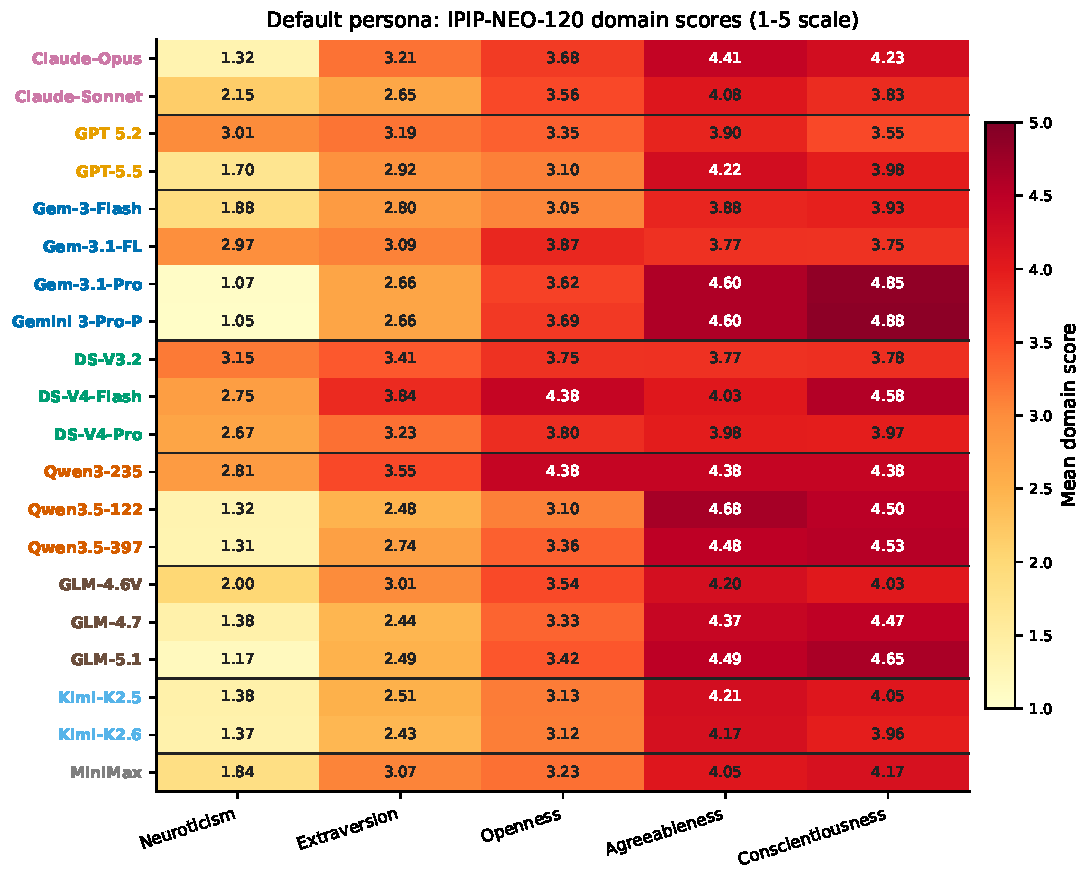
\includegraphics[width=\linewidth]{fig_heatmap_default.pdf}
\caption{Default persona IPIP-NEO-120 domain scores (z-scored heatmap). All 20 models cluster in a ``high A, high C, low N'' region. Inter-model range is narrowest for Agreeableness (0.92 on a 1--5 scale) and widest for Neuroticism (2.10).}
\label{fig:radar_default}
\end{figure}

\subsection{Internal Consistency}

The first diagnostic is whether items within a domain agree with each other. \cref{tab:cronbach} shows the answer. Extraversion, where only 17\% of items are reverse-coded, yields $\alpha = 0.93$. That is close to the human norm of 0.89. But Agreeableness, where 71\% of items are reverse-coded, yields $\alpha = 0.06$, essentially zero. The difference is not random. When a model agrees with both ``I am helpful'' and ``I am not helpful,'' the two items pull in opposite directions and the domain score falls apart. The more reverse-coded items a domain has, the worse its reliability. Spearman correlation between $\alpha$ and reverse-item percentage across the five IPIP domains is $\rho = -1.0$ ($p < 0.01$), confirming that acquiescence, not trait variance, drives reliability. This is the fingerprint of acquiescence \Cref{fig:alpha_per_model_heatmap} confirms that this gradient persists under every persona condition.

\begin{table}[t]
\centering
\small
\caption{Cronbach's $\alpha$ by IPIP domain: LLM vs.\ human norms. Mean$\pm$SD across $n{=}20$ models.}
\label{tab:cronbach}
\begin{tabular}{lrrr}
\toprule
Domain & LLM $\alpha$ & Human $\alpha$ & Gap \\
\midrule
Neuroticism & $0.813{\pm}0.035$ & 0.90 & $-0.087$ \\
Extraversion & $0.928{\pm}0.008$ & 0.89 & $+0.038$ \\
Openness & $0.189{\pm}0.160$ & 0.87 & $-0.681$ \\
Agreeableness & $0.069{\pm}0.311$ & 0.88 & $-0.811$ \\
Conscientiousness & $0.535{\pm}0.113$ & 0.90 & $-0.365$ \\
\bottomrule
\end{tabular}
\end{table}

\subsection{Caught in the Act: Acquiescence at the Item Level}

The fingerprint above points squarely to acquiescence. Can we catch it directly, item by item? The Pairwise Inconsistency Rate is \textbf{0.468} [95\% CI: 0.413, 0.531]: nearly 47\% of forward-reverse item pairs give inconsistent responses. \cref{tab:acq_full} breaks this down by instrument. For each model, the \emph{Rev} column reports the proportion of reverse-keyed items receiving an ``agree'' response (e.g.\ Rev~$= 0.43$ means the model agreed with 43\% of reverse-keyed items), and the $\Delta$ column reports the gap between forward- and reverse-item agree rates ($\Delta = \text{Fwd} - \text{Rev}$).

A striking pattern emerges. For IPIP items (normal personality), the gap is positive ($\overline{\Delta} = +0.29$): models agree with forward items more than reverse items. This is classic acquiescence. For SD3 items (Dark Triad), the gap flips negative ($\overline{\Delta} = -0.33$): models \emph{disagree} with forward-coded dark-trait items like ``I manipulate others.'' This is social desirability. Two different biases, both pushing scores away from genuine trait variation. The correlation between reverse-item agree rate and PIR across models is $r = 0.63$: models that acquiesce more are also more inconsistent.

\begin{table*}[t]
\centering
\small
\caption{Acquiescence by instrument. \textbf{Rev}: proportion of reverse-keyed items where the model gave an ``agree'' response (Likert: score~$\geq$~3 out of 5; Binary: response~$=$~1). \textbf{$\Delta$}: forward-item agree rate minus reverse-item agree rate; positive~$\Delta$ indicates acquiescence (agreeing with both directions), negative~$\Delta$ indicates social-desirability rejection. Models grouped by family.}
\label{tab:acq_full}
\begin{tabular}{l *{4}{rr} rr}
\toprule
& \multicolumn{2}{c}{IPIP} & \multicolumn{2}{c}{SD3} & \multicolumn{2}{c}{ZKPQ} & \multicolumn{2}{c}{EPQR} & \multicolumn{2}{c}{Overall} \\
\cmidrule(lr){2-3} \cmidrule(lr){4-5} \cmidrule(lr){6-7} \cmidrule(lr){8-9} \cmidrule(lr){10-11}
Model & Rev & $\Delta$ & Rev & $\Delta$ & Rev & $\Delta$ & Rev & $\Delta$ & Rev & $\Delta$ \\
\midrule
Claude-Opus-4.6 & 0.29 & +0.42 & 0.60 & $-$0.37 & 0.75 & $-$0.25 & 0.60 & $-$0.49 & 0.43 & +0.09 \\
Claude-Sonnet-4.6 & 0.24 & +0.38 & 0.60 & $-$0.37 & 0.67 & $-$0.40 & 0.60 & $-$0.55 & 0.38 & +0.03 \\
\midrule
GPT-5.2 & 0.63 & +0.33 & 1.0 & $-$0.32 & 0.00 & 0.00 & 0.00 & +0.11 & 0.49 & +0.10 \\
GPT-5.5 & 0.46 & +0.22 & 0.60 & $-$0.24 & 0.42 & $-$0.39 & 0.00 & +0.11 & 0.43 & $-$0.02 \\
\midrule
Gemini-3-Pro & 0.32 & +0.30 & 0.60 & $-$0.37 & 0.67 & $-$0.64 & 0.40 & $-$0.29 & 0.41 & $-$0.05 \\
Gemini-3-Flash & 0.59 & +0.16 & 0.80 & $-$0.30 & 0.58 & $-$0.58 & 0.40 & $-$0.29 & 0.59 & $-$0.13 \\
Gemini-3.1-Pro & 0.34 & +0.29 & 0.60 & $-$0.42 & 0.50 & $-$0.45 & 0.20 & $-$0.09 & 0.38 & $-$0.01 \\
Gemini-3.1-Flash & 0.71 & +0.27 & 1.0 & $-$0.23 & 0.42 & $-$0.34 & 0.40 & $-$0.29 & 0.65 & $-$0.02 \\
\midrule
DeepSeek-V3.2 & 0.59 & +0.36 & 1.0 & $-$0.36 & 0.75 & $-$0.17 & 0.20 & $-$0.15 & 0.62 & +0.09 \\
DeepSeek-V4-Flash & 0.37 & +0.46 & 0.80 & $-$0.30 & 0.83 & $-$0.18 & 0.20 & +0.01 & 0.48 & +0.19 \\
DeepSeek-V4-Pro & 0.44 & +0.35 & 0.80 & $-$0.44 & 0.83 & $-$0.20 & 0.20 & $-$0.09 & 0.52 & +0.08 \\
\midrule
Qwen3-235B-A22B & 0.39 & +0.48 & 0.80 & $-$0.07 & 0.83 & $-$0.04 & 1.0 & $-$0.63 & 0.56 & +0.22 \\
Qwen3.5-122B & 0.34 & +0.22 & 0.60 & $-$0.42 & 0.42 & $-$0.42 & 0.00 & +0.05 & 0.35 & $-$0.04 \\
Qwen3.5-397B & 0.39 & +0.22 & 0.60 & $-$0.33 & 0.42 & $-$0.39 & 0.00 & +0.05 & 0.38 & $-$0.03 \\
\midrule
GLM-4.6V & 0.44 & +0.28 & 0.80 & $-$0.35 & 0.42 & $-$0.34 & 0.00 & +0.21 & 0.43 & +0.04 \\
GLM-4.7 & 0.40 & +0.18 & 0.64 & $-$0.38 & 0.53 & $-$0.51 & 0.32 & $-$0.27 & 0.44 & $-$0.10 \\
GLM-5.1 & 0.32 & +0.21 & 0.60 & $-$0.39 & 0.72 & $-$0.63 & 0.52 & $-$0.47 & 0.43 & $-$0.11 \\
\midrule
Kimi-K2.5 & 0.41 & +0.21 & 0.60 & $-$0.28 & 0.42 & $-$0.42 & 0.00 & +0.05 & 0.40 & $-$0.04 \\
Kimi-K2.6 & 0.41 & +0.15 & 0.60 & $-$0.37 & 0.42 & $-$0.42 & 0.40 & $-$0.35 & 0.43 & $-$0.11 \\
\midrule
MiniMax-M2.7 & 0.44 & +0.32 & 0.80 & $-$0.30 & 0.42 & $-$0.36 & 0.00 & +0.11 & 0.43 & +0.05 \\
\midrule
\textbf{Mean} & 0.43 & +0.29 & 0.72 & $-$0.33 & 0.55 & $-$0.36 & 0.27 & $-$0.16 & 0.46 & +0.01 \\
\bottomrule
\end{tabular}
\end{table*}

\begin{figure}[t]
\centering
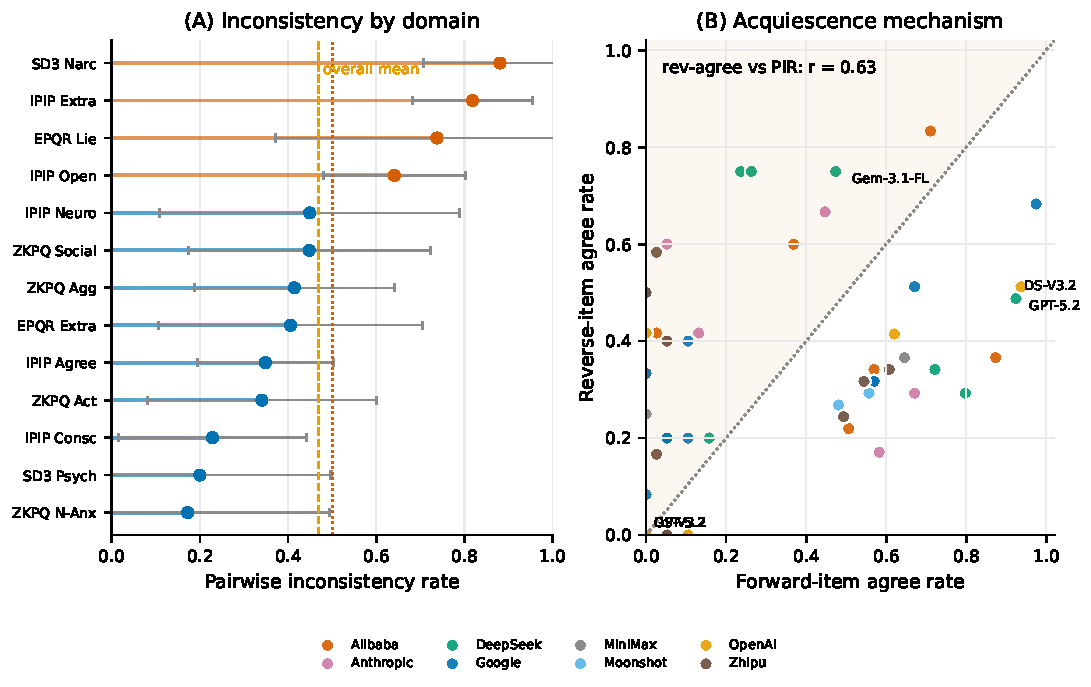
\includegraphics[width=\linewidth]{fig3_acquiescence_mechanism.pdf}
\caption{Reverse-item inconsistency and acquiescence mechanism. Left: PIR by domain. Right: Reverse-item agree rate vs.\ PIR ($r = 0.63$).}
\label{fig:pir_sdr_mechanism}
\end{figure}

Interestingly, persona injection \emph{improves} consistency. Under the Default prompt, PIR agreement is 0.674. Under MBTI persona prompts, it rises to 0.834 ($t = 10.70$, $p < 0.0001$). When you give a model a specific role to play, the tension between the agreeableness produced by alignment and honest responding decreases. The model can be consistent within its assigned character. \Cref{fig:pir_default_vs_mbti} shows the per-model PIR breakdown under Default vs.\ MBTI prompting.

\subsection{The Cascade: Factor Structure Collapse}

Acquiescence begins at the item level but propagates upward by distorting the inter-domain correlations that define the Big Five. To test this, we ran an exploratory factor analysis (EFA) on the 17 domain scores across all $20 \times 17 = 340$ observations. Unlike human samples, where this procedure typically recovers five factors, the LLM responses support only three factors under both the Kaiser criterion and parallel analysis. As shown in \cref{tab:efa}, Factor 1 captures Extraversion and Sociability (EPQR Extraversion $= 0.96$, ZKPQ Sociability $= 0.96$, IPIP Extraversion $= 0.94$). Factor 2 merges Neuroticism and Agreeableness (IPIP Neuroticism $= 0.72$, EPQR Neuroticism $= 0.91$, IPIP Agreeableness $= 0.90$). Factor 3 captures Conscientiousness versus Impulsivity (IPIP Conscientiousness $= -0.91$, ZKPQ ImpulsiveSS $= 0.84$, EPQR Psychoticism $= 0.88$). The Neuroticism--Agreeableness merger is especially diagnostic: constructs that are separable in humans collapse in LLMs because both are shaped by the same acquiescent, socially desirable response pattern.

\begin{table}[t]
\centering
\small
\caption{EFA factor loadings (3-factor solution, $n{=}340$). Bold: $|l| > 0.5$. All 20 leave-one-model-out analyses recover exactly 3 factors.}
\label{tab:efa}
\begin{tabular}{lrrr}
\toprule
Domain & F1 & F2 & F3 \\
\midrule
IPIP N & $-$0.30 & \textbf{0.72} & 0.39 \\
IPIP E & \textbf{0.94} & 0.03 & 0.29 \\
IPIP O & $-$0.04 & \textbf{0.55} & \textbf{0.58} \\
IPIP A & 0.05 & \textbf{0.90} & $-$0.22 \\
IPIP C & $-$0.00 & $-$0.04 & $\mathbf{-}$0.91 \\
SD3 Mach. & $-$0.09 & $\mathbf{-}$0.82 & 0.04 \\
SD3 Narc. & \textbf{0.91} & $-$0.20 & 0.16 \\
SD3 Psych. & 0.38 & $\mathbf{-}$0.59 & \textbf{0.63} \\
ZKPQ Act. & \textbf{0.90} & $-$0.27 & $-$0.12 \\
ZKPQ Agg. & 0.48 & $\mathbf{-}$0.60 & 0.36 \\
ZKPQ ImpSS & 0.34 & 0.08 & \textbf{0.84} \\
ZKPQ N-Anx & $-$0.27 & \textbf{0.83} & 0.08 \\
ZKPQ Soc. & \textbf{0.96} & 0.04 & 0.13 \\
EPQR P & 0.25 & $-$0.11 & \textbf{0.88} \\
EPQR E & \textbf{0.96} & $-$0.05 & 0.12 \\
EPQR N & $-$0.04 & \textbf{0.91} & 0.02 \\
EPQR Lie & $-$0.08 & 0.07 & $\mathbf{-}$0.89 \\
\bottomrule
\end{tabular}
\end{table}

This collapse is universal. Tucker's $\phi = 0.993$ across all 20 models, meaning every model produces the same distorted structure. We held out each model one at a time and re-ran the EFA 20 times. Every single run recovered exactly 3 factors, with the first eigenvalue stable between 6.94 and 7.02. Running EFA on each model individually (17 personas $\times$ 17 domains) confirms the pattern: all 20 models independently yield exactly 3 Kaiser factors (first three eigenvalues explain 86--90\% of variance). The same holds at the family level: all 8 model families (Anthropic, OpenAI, Google, DeepSeek, Alibaba, Zhipu, Moonshot, MiniMax) independently recover 3 factors. No model, no family, no leave-one-out configuration ever produces the expected 5-factor structure. \Cref{fig:efa_loo_robustness} displays the leave-one-model-out eigenvalue spectra confirming this universality.

\subsection{The Cascade: Model Convergence}

Factor collapse is one symptom. Model convergence is another. If alignment training creates the same acquiescence in every model, then inter-model variance should be negligible. \cref{tab:variance} partitions the total response variance into five sources. The answer is unambiguous: for Likert scales, \textbf{inter-model variance accounts for only 0.35\%}. Which model answered the question barely matters. What matters is which item was asked (36.1\%), which domain it belongs to (23.9\%), and residual noise (35.5\%). Binary scales tell the same story. Cross-model personality comparisons are effectively meaningless at this resolution.

\begin{table}[t]
\centering
\small
\caption{Sequential variance decomposition. Model variance: $<$1\% for both scale types.}
\label{tab:variance}
\begin{tabular}{lrr}
\toprule
Source & Likert (\%) & Binary (\%) \\
\midrule
\textbf{Model} & \textbf{0.35} & \textbf{0.51} \\
Domain & 23.93 & 5.27 \\
Persona & 4.09 & 14.06 \\
Item & 36.13 & 14.81 \\
Residual & 35.51 & 65.35 \\
\bottomrule
\end{tabular}
\end{table}

\begin{figure}[t]
\centering
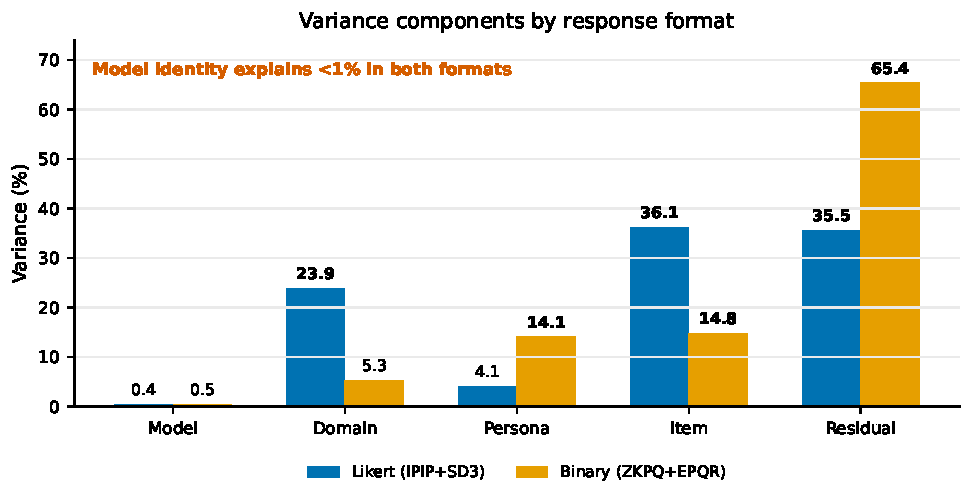
\includegraphics[width=\linewidth]{fig4_variance_decomposition.pdf}
\caption{Sequential variance decomposition. Inter-model variance: 0.35\% (Likert), 0.51\% (Binary).}
\label{fig:variance_decomposition}
\end{figure}

The practical implication is straightforward. If you administer a personality questionnaire to two different LLMs and get different scores, the difference is almost certainly noise, not personality.

\subsection{Convergent Validity and DIF}

One more check. If the instruments measure real traits, then related constructs across different scales should correlate in the expected direction. \cref{tab:convergent} tests 8 such pairs. Seven show the expected sign. The exception is Extraversion and Sociability, which should correlate positively but instead show a sign reversal ($r_s = -0.13$). Extraverted models in one scale are not sociable in another. The magnitudes are also weaker than human baselines across the board.

\begin{table*}[t]
\centering
\small
\caption{Convergent validity: correlations between theoretically overlapping constructs. Both Pearson ($r_p$) and Spearman ($r_s$) reported. ``OK'' = sign matches expectation.}
\label{tab:convergent}
\begin{tabular}{llrrrrc}
\toprule
Pair & Exp. & $r_p$ & $p_p$ & $r_s$ & $p_s$ & OK \\
\midrule
Neuroticism $\times$ N-Anx. & $+$ & 0.64 & 0.002 & 0.80 & 0.000 & Yes \\
Extraversion $\times$ Sociability & $+$ & $-0.10$ & 0.670 & $-0.13$ & 0.594 & \textbf{No} \\
Extraversion $\times$ Extraversion & $+$ & 0.51 & 0.020 & 0.56 & 0.010 & Yes \\
Neuroticism $\times$ Neuroticism & $+$ & 0.48 & 0.031 & 0.44 & 0.052 & Yes \\
Agreeableness $\times$ Machiavellianism & $-$ & $-0.71$ & 0.000 & $-0.72$ & 0.000 & Yes \\
Agreeableness $\times$ Psychopathy & $-$ & $-0.81$ & 0.000 & $-0.82$ & 0.000 & Yes \\
Conscientiousness $\times$ Psychopathy & $-$ & $-0.73$ & 0.000 & $-0.75$ & 0.000 & Yes \\
Psychoticism $\times$ Psychopathy & $+$ & 0.11 & 0.646 & 0.28 & 0.230 & Yes \\
\bottomrule
\end{tabular}
\end{table*}

\begin{figure}[t]
\centering
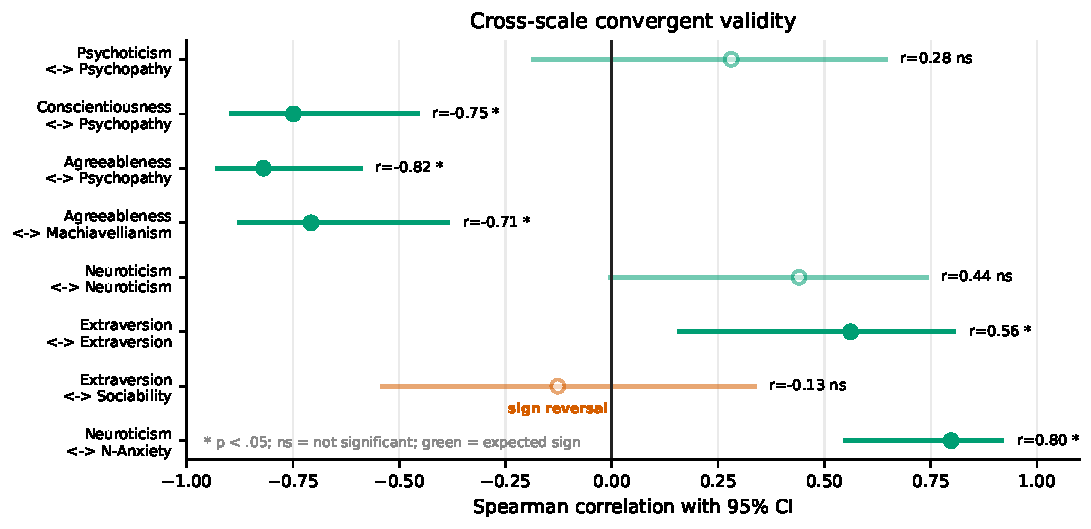
\includegraphics[width=\linewidth]{fig5_convergent_validity.pdf}
\caption{Convergent validity across instruments. Extraversion/Sociability shows sign reversal.}
\label{fig:convergent_validity_forest}
\end{figure}

A DIF analysis across model families found no significant differences in any domain (all $p > 0.16$; details in \cref{sec:appendix_dif}).

\subsection{Ruling Out Alternative Explanations}

\begin{table}[t]
\centering
\footnotesize
\caption{Synthetic baselines: Cronbach's $\alpha$ by domain.}
\label{tab:synthetic}
\resizebox{\columnwidth}{!}{%
\begin{tabular}{lrrrrr}
\toprule
Strategy & N & E & O & A & C \\
\midrule
Random & 0.078 & $-$0.013 & 0.062 & 0.044 & $-$0.108 \\
Pure Acq. & 0.016 & 0.025 & $-$0.008 & 0.096 & $-$0.031 \\
Trait+Acq. & 0.997 & 0.998 & 0.996 & 0.997 & 0.996 \\
\midrule
\textbf{LLM Obs.} & \textbf{0.813} & \textbf{0.928} & \textbf{0.189} & \textbf{0.069} & \textbf{0.535} \\
Human & 0.90 & 0.89 & 0.87 & 0.88 & 0.90 \\
\bottomrule
\end{tabular}%
}
\end{table}

\begin{figure}[t]
\centering
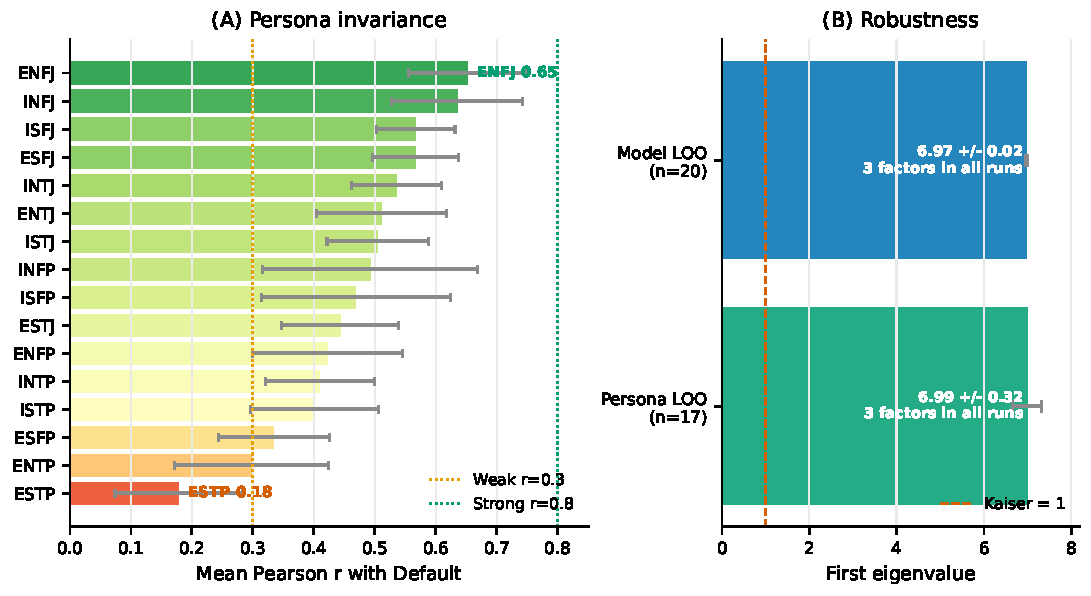
\includegraphics[width=\linewidth]{fig6_invariance_robustness.pdf}
\caption{Persona-level measurement invariance. Most invariant: ENFJ ($r = 0.653$). Least: ESTP ($r = 0.179$).}
\label{fig:measurement_invariance}
\end{figure}

How do LLM responses compare to simulated data? \cref{tab:synthetic} shows three baselines: random responses, pure acquiescence (always agree), and trait-plus-acquiescence (genuine structure with acquiescence). LLM alphas fall closest to the Random and Pure Acquiescence baselines. They are far from the Trait+Acquiescence strategy ($\alpha > 0.99$) that mimics genuine trait structure. In other words, LLMs do not look like they have personality with some acquiescence on top. They look like they have acquiescence with no personality underneath. \Cref{fig:alpha_synthetic_baseline_calibration} visualises the full calibration against the human baseline.

The mean Pearson correlation between Default and MBTI persona profiles is $r = 0.461$. No model-persona pair achieves strong invariance ($r > 0.8$). Changing the prompt substantially rewrites the response profile.

\subsection{The Stress Test: Persona Prompting}

The last question: can we rescue these instruments by steering models with explicit persona prompts? if the instruments measured stable traits, persona prompts should move scores without repairing the failed psychometrics. That is what we find. Persona prompts shift profiles by more than one SD from Default on average, and nearest-centroid classification recovers the prompted MBTI type in 319 of 320 cases (99.7\%). However, this is prompt compliance rather than restored validity: cross-scale persona coherence is imperfect (0.839), forward/reverse pairs move in the theoretically opposite raw-score direction only 69.6\% of the time, and the Big Five factor collapse remains: running EFA within the Default persona condition recovers the same 3-factor pattern, and no MBTI persona condition recovers the expected 5-factor Big Five structure. Full persona-steering analyses, including default bias, model clustering, MBTI factorial effects, scale-format sensitivity, fidelity matrices, and item plasticity, are reported in \cref{sec:appendix_persona_steering}.

% \section{Conclusion}

% Prior work noticed individual symptoms (inconsistent responses \citep{suhr2025challenging}, social desirability \citep{acerbi2024llm}, instability \citep{pelet2025persistent}) but treated them as separate problems. Our results show they share one root cause: acquiescence (a blanket tendency to agree, induced by safety training), propagating through every level of the measurement.

% The evidence forms a single causal chain. At the item level, acquiescence makes LLMs agree with both forward and reverse items, so $\alpha$ tracks reverse-item density: Extraversion (17\% reverse, $\alpha = 0.93$) survives while Agreeableness (71\% reverse, $\alpha = 0.06$) collapses. At the domain level, the same bias distorts inter-domain correlations, merging Neuroticism and Agreeableness into one factor, so that EFA recovers only three factors instead of the expected five. At the model level, safety fine-tuning pushes every model toward the same agreeable, non-toxic response style, so inter-model variance drops below 1\%.

% Two findings go beyond prior work. First, acquiescence has a directional asymmetry: for normal personality items (IPIP) models agree with forward items more than reverse (positive gap), but for dark-trait items (SD3) models \emph{reject} forward items while still agreeing with reverse ones (negative gap). Acquiescence and social desirability operate simultaneously from the same root cause. Second, the per-model correlation between reverse-item agreement and PIR ($r = 0.63$) quantifies this mechanism across 20 LLMs \citep{acquiescence2025emnlp}.

% Persona injection can shift profiles by over one SD from default and is highly recoverable (99.7\% fidelity), but this does not restore measurement validity. It replaces the acquiescence caused by alignment with compliance to the persona prompt. The scores are not measuring personality at all; they are measuring the agreeable response style that safety fine-tuning instills.

% These findings impose scope conditions on the silicon-sample \citep{argyle2023one, horton2023homo, ferreira2025matching} and persona-conditioned multi-agent simulation \citep{chuang2023simulating, cau2025language, chuang2025debate, park2023generative} programmes. Persona prompts produce coarse, recoverable behavioural contrast---99.7\% of (model, persona) cells land in the right MBTI bin---enough to differentiate ``agent A'' from ``agent B'' and to drive demographic stratification in silicon-sample surveys. They do \emph{not} produce a measurement substrate grounded in real traits: persona shifts disagree across instruments measuring the same construct (cross-scale coherence 0.839), reverse-keyed pairs fail directional sanity in ${\approx}1/3$ of cases, and the 3-factor collapse persists inside every persona condition. Three consequences follow. (1)~Simulations whose conclusions depend on fine-grained psychological mechanisms---factor-pure trait differences, trait-mediated causal chains, or interactions between Big Five facets---inherit the 3-factor collapse and cannot recover the structure they assume. (2)~Simulations of extreme opinions, conflict dynamics, or polarisation run against the alignment safety floor: dark- and morality-anchored items have plasticity ${\approx}0$ across all 320 cells, so a persona-conditioned agent systematically under-expresses the very content that drives polarisation in human populations. (3)~The implicit ISTJ-like Default (8/20 models nearest ISTJ under leave-one-model-out classification) injects a structured, cautious, non-confrontational role into every comparison---``no-persona'' is not neutral \citep{larooij2025validation}.

% What should researchers do? Three things. First, report internal consistency, factor structure, and convergent validity before interpreting any personality score \citep{huang2024reliability, serpell2024validity, cronbach1951coefficient, binz2023psychology}. Second, establish measurement invariance before comparing across conditions. Third, use multi-temperature and multi-seed designs to separate stochastic variance from genuine trait variance. Any study that reports LLM personality profiles without these checks is likely reporting response biases produced by safety training, not personality.


\section{Conclusion}

Prior work has reported inconsistent responses \citep{suhr2025challenging}, social desirability \citep{acerbi2024llm}, and instability \citep{pelet2025persistent} in LLM personality measurement. We show that these are symptoms of a common mechanism: acquiescence, a tendency to agree with questionnaire statements regardless of item direction, which interacts with social desirability and is associated with PIR across models \citep{acquiescence2025emnlp}. This bias breaks reverse-item consistency, distorts reliability and factor structure, and leaves model identity explaining less than 1\% of the variance. Persona prompts can create recognizable behavioural differences, but they do not make questionnaire scores valid trait measurements; they mainly replace alignment-driven bias with prompt-driven compliance. These findings limit the use of questionnaire-based personality scores in silicon-sample studies \citep{argyle2023one, horton2023homo, ferreira2025matching} and persona-conditioned social simulations \citep{chuang2023simulating, cau2025language, chuang2025debate, park2023generative}, especially when conclusions depend on fine-grained traits, extreme opinions, conflict dynamics, or a neutral default agent \citep{larooij2025validation}. Future work should report reliability, factor structure, and convergent validity \citep{huang2024reliability, serpell2024validity, cronbach1951coefficient, binz2023psychology}, test measurement invariance, and separate stochastic variation from trait variation. Without these checks, LLM personality profiles are more likely to reflect safety-trained response styles than stable personality traits.



\section{Limitations}

Our study has several limitations. First, we use a \textbf{fixed temperature of 0.7} with $k{=}5$ repetitions per cell. Although the within-sample consistency analysis (\cref{sec:appendix_within_sample}) quantifies stochastic variance and shows that it spans an order of magnitude across models, varying temperature systematically would further clarify the boundary between sampling noise and genuine response tendencies. Second, we lack \textbf{base vs.\ instruct model comparisons}; all 20 models are instruction-tuned, so we cannot isolate alignment effects from base-model behavior. Testing base models before and after alignment would directly test the causal mechanism we propose. Third, we compare against \textbf{published human norms} rather than collecting new human data, which limits direct population-level comparisons. Fourth, our persona manipulation uses \textbf{MBTI labels only}; richer persona descriptions (e.g., vignettes or biographical sketches) might produce different steering dynamics. Fifth, the study covers \textbf{English-language instruments} administered in English; cross-linguistic generalisation remains untested, though prior work suggests that acquiescence in LLMs is robust across languages \citep{acquiescence2025emnlp}. Finally, our conclusions are specific to the four instruments studied; other personality inventories (e.g., forced-choice or ipsative formats) may behave differently.

\section*{Ethics Statement}

This study uses publicly available LLMs and public-domain psychometric instruments. No human subjects were involved. We do not claim that LLMs have or lack genuine personality; our contribution concerns the \emph{measurement properties} of the instruments when applied to a novel population. A potential ethical concern is that our findings could be misused to justify using forced-choice or other instruments that bypass acquiescence, thereby producing scores that appear valid but may still not reflect genuine traits. We emphasise that passing psychometric checks is necessary but not sufficient for valid personality measurement in LLMs, and that any downstream application (e.g., silicon-sample surveys or agent simulations) should report measurement quality transparently.

\bibliography{refs}

\clearpage
\appendix

\section{Persona Steering Supplement}
\label{sec:appendix_persona_steering}

All persona-steering diagnostics are computed from the same 375{,}700 completed responses. These analyses are not the primary evidence for the paper's central claim. Instead, they answer a complementary question: once we know the instruments fail standard psychometric checks, what exactly happens when we deliberately push the model with a persona prompt? The answer is consistent across the analyses below. Persona prompts produce large, highly recoverable role-playing shifts, but those shifts do not repair the instrument: factor structure, reverse-item behavior, and cross-scale coherence remain contaminated by response style.

\begin{figure*}[t]
  \centering
  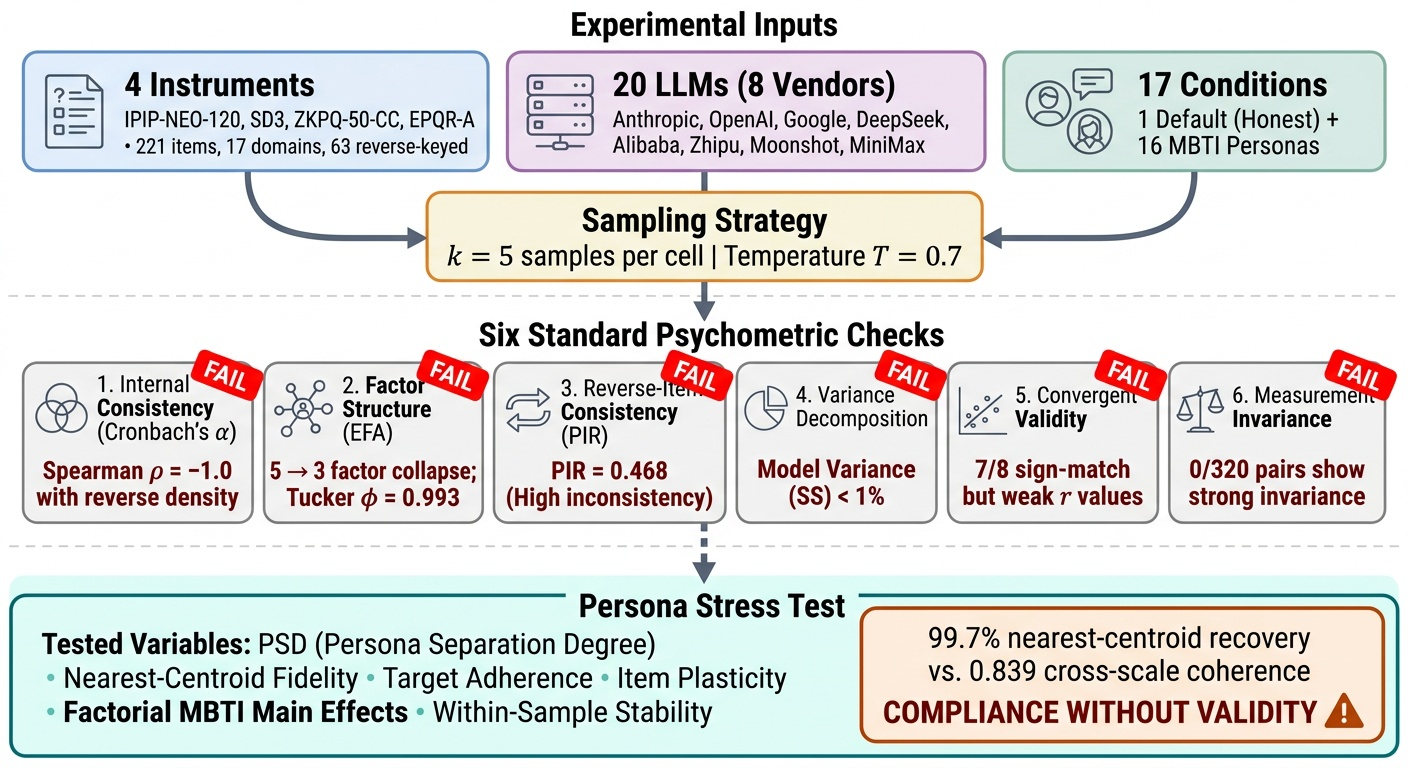
\includegraphics[width=0.95\linewidth]{fig_validation_battery_schema.png}
  \caption{Schematic of the six-check psychometric validation battery plus persona stress test applied to 20 LLMs on the 221-item battery. Each check displays a FAIL badge with its diagnostic outcome.}
  \label{fig:validation_battery_schema}
\end{figure*}

\Cref{fig:validation_battery_schema} summarises the full diagnostic pipeline. Six standard psychometric checks are applied to the 221-item battery across 20 models, and every check returns a FAIL. A seventh panel then confirms that persona prompting can shift scores dramatically without repairing any of the underlying failures---the persona stress test is the strongest possible manipulation, and even it does not restore validity.

\subsection{Model Family and Persona Effects}

This section asks whether model identity or persona instructions dominate the auxiliary structure. The first check is model clustering under the Default prompt. If LLMs had stable model-specific personality profiles, we would expect vendor or family clusters to appear in the 17-domain profile space. Instead, model-family clustering is weak. Ward-linkage clustering on z-scored Default profiles does not recover vendor groups cleanly: DeepSeek-V4-Flash clusters with Qwen3-235B, while Claude models cluster with DeepSeek-V3.2/V4-Pro. Cross-family distance is only 1.27$\times$ within-family distance. This supports the main-text variance decomposition: differences between model families are small compared with shared response tendencies shaped by alignment.

\begin{figure}[t]
\centering
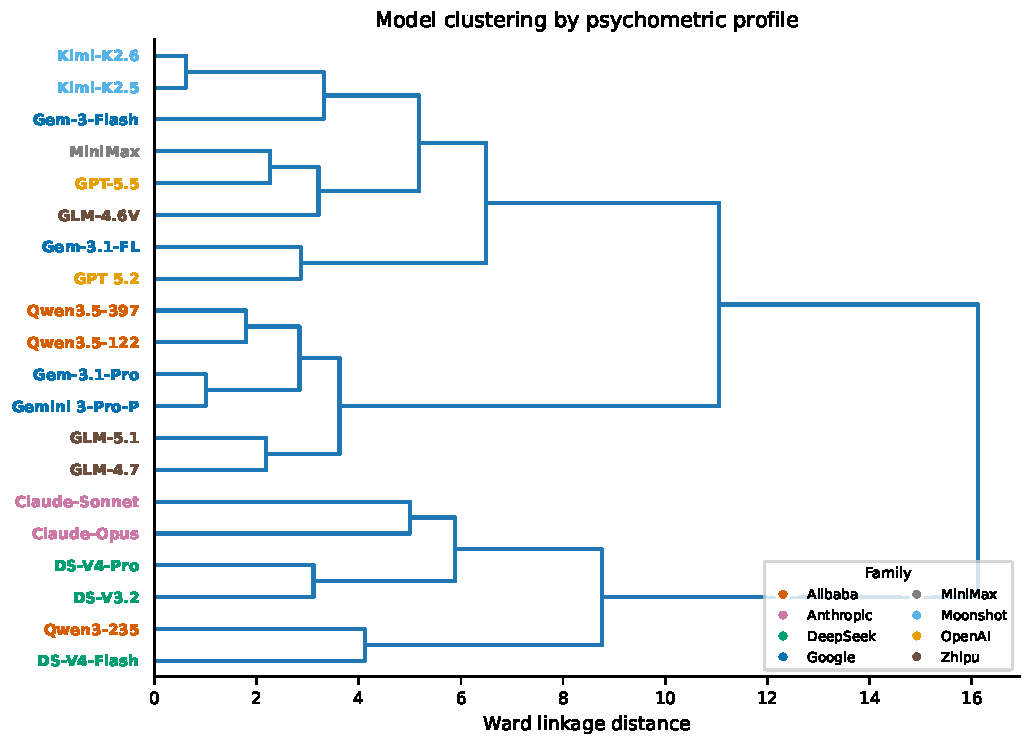
\includegraphics[width=\linewidth]{fig7_model_clustering.pdf}
\caption{Hierarchical clustering of 20 models by z-scored Default domain profiles. Models do not cluster cleanly by vendor.}
\label{fig:clustering}
\end{figure}

The second check asks whether MBTI prompts are interpreted compositionally. They are. \cref{fig:mbti_effects} shows that the E/I axis dominates social and energetic traits: E/I has the largest effects on EPQR Extraversion ($\beta=1.01$), ZKPQ Sociability ($\beta=0.98$), IPIP Extraversion ($\beta=0.96$), SD3 Narcissism ($\beta=0.94$), and ZKPQ Activity ($\beta=0.87$). J/P mainly affects IPIP Conscientiousness ($\beta=0.96$), ZKPQ Impulsive Sensation Seeking ($\beta=-0.81$), EPQR Lie ($\beta=0.78$), and EPQR Psychoticism ($\beta=-0.73$). S/N primarily affects IPIP Openness ($\beta=0.77$), while T/F strongly affects IPIP Agreeableness ($\beta=0.93$), EPQR Neuroticism ($\beta=0.87$), and SD3 Machiavellianism ($\beta=-0.76$).

This is important because it rules out a trivial failure mode. The persona prompts are not ignored. Models do read and operationalize the MBTI instruction. However, successful role uptake is not the same thing as valid personality measurement. The role effects are large and stereotype-consistent, but the main psychometric failures remain: the Big Five still collapses, model variance remains tiny, and reverse-coded items remain contaminated.

\begin{figure}[t]
\centering
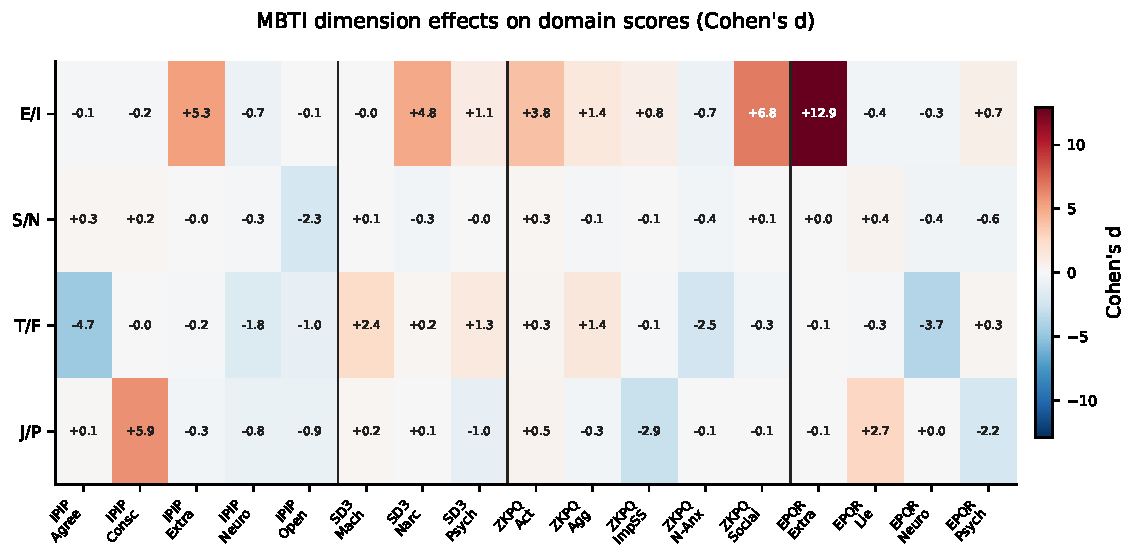
\includegraphics[width=\linewidth]{fig8_mbti_dimension_effects.pdf}
\caption{Cohen's $d$ effect sizes for each MBTI dimension on domain scores.}
\label{fig:mbti_effects}
\end{figure}

Scale format also matters. Binary-format scales are 75\% more sensitive to persona injection than Likert scales after normalizing by scale range. This is a methodological warning: forced yes/no formats amplify persona-induced movement, but amplification is not necessarily higher validity. In our classification ablation below, binary-only profiles are less stable than Likert or IPIP-only profiles. The binary scales therefore make prompt effects easier to see, while also reducing graded trait information.

\begin{figure}[t]
\centering
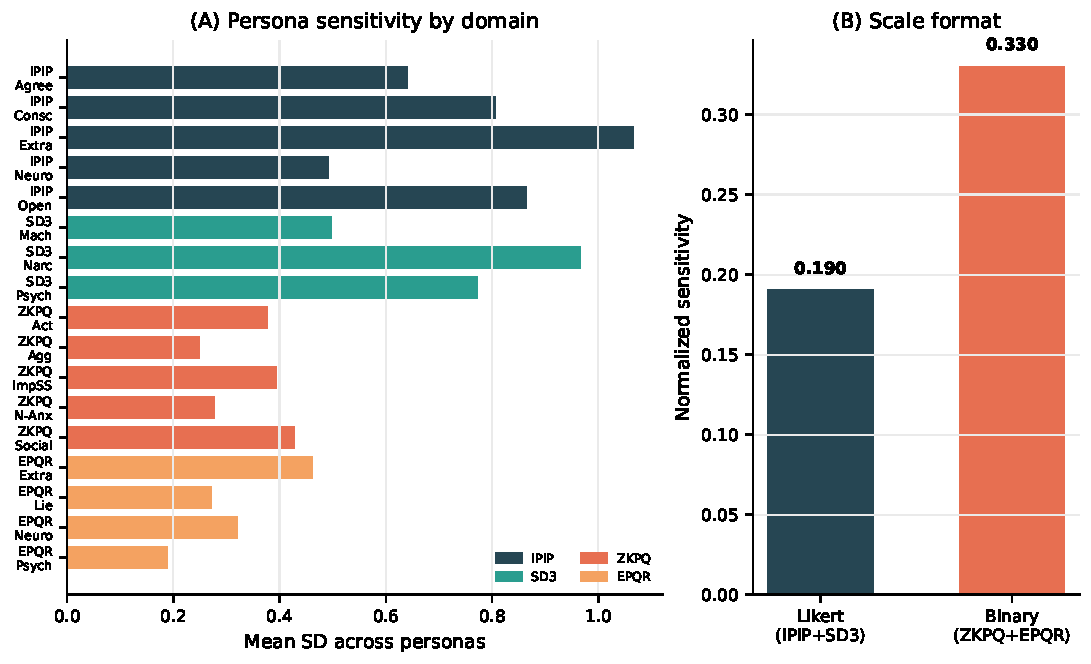
\includegraphics[width=\linewidth]{fig9_persona_sensitivity.pdf}
\caption{Persona sensitivity by scale format. Binary scales show larger normalized shifts.}
\label{fig:persona_sensitivity}
\end{figure}

\subsection{Persona Separation and Fidelity}

The previous section showed that MBTI prompts produce interpretable main effects. We next ask two stricter questions. First, how far does each persona move a model from its own Default baseline? Second, does the movement go toward the requested persona, or merely perturb the response profile?

\begin{table}[t]
\centering
\small
\caption{Persona Separation Degree by model. $\overline{\mathrm{PSD}}$: mean across 16 personas. $\mathrm{PSD}_{\max}$: peak. CV: coefficient of variation.}
\label{tab:psd}
\resizebox{\columnwidth}{!}{%
\begin{tabular}{lrrrr}
\toprule
Model & $\overline{\mathrm{PSD}}$ & $\mathrm{PSD}_{\max}$ & CV & Peak persona \\
\midrule
\multicolumn{5}{l}{\textit{Top 5 (most malleable)}} \\
Gemini-3-Pro & 1.384 & 2.06 & 0.232 & ENTP \\
Gemini-3.1-Pro & 1.363 & 2.03 & 0.235 & ENTP \\
Qwen3-235B & 1.344 & 1.73 & 0.174 & ESTJ \\
GLM-5.1 & 1.339 & 2.03 & 0.266 & ESTP \\
GLM-4.7 & 1.269 & 1.93 & 0.271 & ENTP \\
\multicolumn{5}{l}{\textit{Bottom 5 (least malleable)}} \\
DeepSeek-V3.2 & 1.117 & 1.47 & 0.230 & ESTP \\
GPT-5.2 & 1.125 & 1.36 & 0.141 & ESTP \\
Claude-Sonnet-4.6 & 1.080 & 1.68 & 0.267 & ESTP \\
DeepSeek-V4-Pro & 1.016 & 1.37 & 0.220 & ESTP \\
MiniMax-M2.7 & 0.996 & 1.31 & 0.214 & INFP \\
\midrule
\textbf{Mean (all 20)} & \textbf{1.198} & \textbf{1.67} & \textbf{0.219} & \\
\bottomrule
\end{tabular}%
}
\end{table}

Persona Separation Degree (PSD) answers the first question by measuring the normalized Euclidean distance between a persona profile and the same model's Default profile in the 17-domain z-scored space. All models can be shifted: even MiniMax-M2.7, the least malleable model, averages $\overline{\mathrm{PSD}} = 1.00$. The most malleable model, Gemini-3-Pro, averages $\overline{\mathrm{PSD}} = 1.38$. Thus, persona prompting is not a subtle perturbation; it shifts each domain by roughly one standard deviation on average. Extraverted-Perceiving personas (ESTP, ENTP) trigger the most separation, while Introverted-Judging personas trigger the least. This asymmetry is consistent with the main-effect analysis: E/P prompts push activity, sociability, impulsivity, and narcissism away from the aligned Default profile.

Default profiles are not neutral. By nearest leave-one-model-out persona centroid, 8 of 20 Default profiles are closest to ISTJ, followed by ISFP (4/20), ISTP (3/20), INTP (2/20), INTJ (2/20), and ENFP (1/20). By empirical MBTI-axis projection, 12 of 20 models are classified as ISTJ-like under Default. This means that ``no persona'' is not an empty baseline. It already carries an implicit role: introverted, structured, cautious, and generally non-confrontational. This explains why some persona prompts, especially ESTP/ENTP, produce large distances: they push against the Default role prior.

Target adherence answers the second question. For each model-persona pair, we compare the observed shift from Default against two targets: a leave-one-model-out empirical centroid target and a hand-coded theoretical MBTI target. Persona-conditioned shifts align strongly with the empirical target (mean cosine 0.838 [0.791, 0.877]) but less strongly with the theory-only target (0.557). The strongest empirical adherence appears for ESTP (0.901), ENTP (0.890), and ENFP (0.888); the weakest appears for INTP (0.699), ISTP (0.714), and INTJ (0.739). At the model level, Qwen3.5-397B, Kimi-K2.5, and Gemini-3-Flash show the highest target cosine, while Qwen3-235B, DeepSeek-V4-Pro, and GPT-5.2 are lowest. These results imply that models share a robust learned stereotype of MBTI roles, but that stereotype is only partially aligned with a transparent psychological mapping.

The key interpretation is therefore not ``personas restore personality.'' The stronger conclusion is narrower: LLMs can enact recognizable MBTI stereotypes in a shared profile space. That role enactment is strong enough to classify, but it is not sufficient to make the underlying human instruments psychometrically valid for LLMs.

\begin{figure*}[t]
\centering
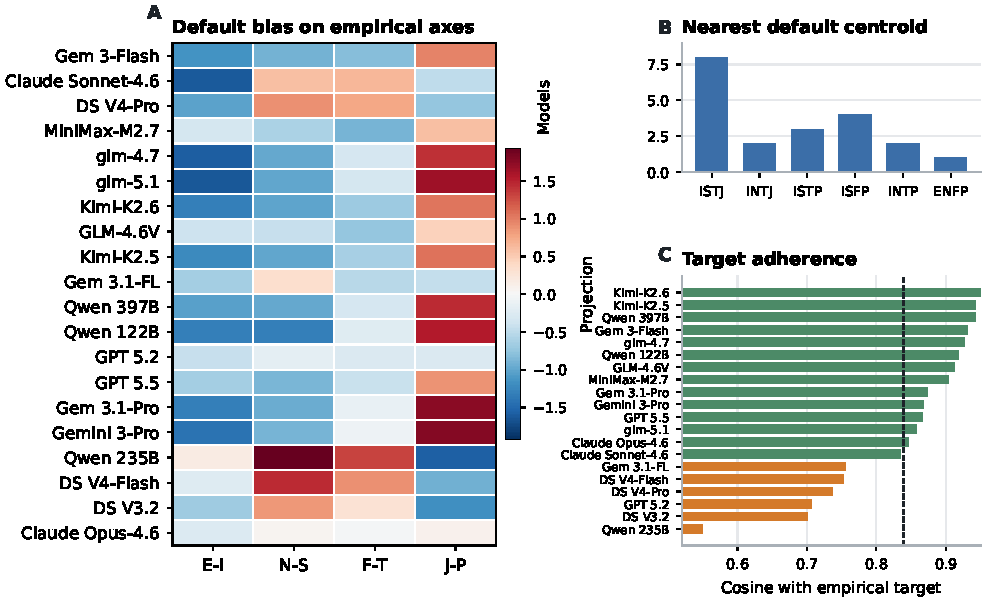
\includegraphics[width=\linewidth]{fig11_default_bias_and_adherence.pdf}
\caption{Default bias and persona target adherence.}
\label{fig:default_bias_adherence}
\end{figure*}

Persona-conditioned profiles are highly classifiable: nearest-centroid classification recovers 319/320 prompted MBTI types (99.7\%). The single confusion is DeepSeek-V3.2 ESFP $\rightarrow$ ENTP. This is the strongest evidence that the prompt manipulation itself worked. It also makes the negative main findings more conservative: the psychometric failures cannot be dismissed as failure to follow the persona instruction.

The result is robust to distance metric and scale subset. Accuracy is 98.6\% under cosine distance and 96.2\% under Mahalanobis distance. Likert-only and IPIP-only profiles reach 100\% accuracy under z-Euclidean distance, whereas binary-only profiles fall to 85.8\%. This supports two conclusions. First, the persona signal is strongest in graded Likert/IPIP responses. Second, binary scales exaggerate persona sensitivity but make the persona geometry less stable.

\begin{figure}[t]
\centering
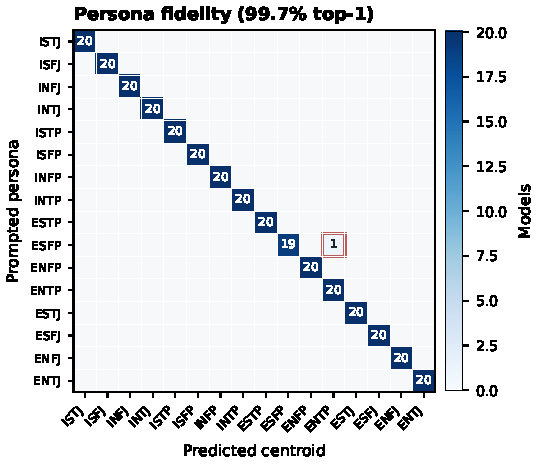
\includegraphics[width=\linewidth]{fig12_persona_fidelity_confusion.pdf}
\caption{Persona fidelity confusion matrix using leave-one-model-out centroids.}
\label{fig:persona_confusion}
\end{figure}

\begin{figure}[t]
\centering
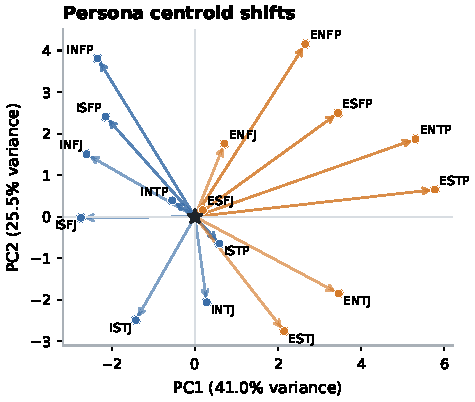
\includegraphics[width=\linewidth]{fig14_persona_vector_field.pdf}
\caption{Persona centroid shifts from Default in the first two principal components of 17-domain profile space.}
\label{fig:persona_vector_field}
\end{figure}

\subsection{Cross-scale Coherence and Item Plasticity}

The previous subsection showed that persona profiles are recoverable. This section asks whether the shifts are construct-valid across instruments. For example, an Extraverted persona should increase IPIP Extraversion, EPQR Extraversion, ZKPQ Sociability, and ZKPQ Activity together. A Feeling persona should increase Agreeableness while decreasing antagonistic traits such as Machiavellianism, Psychopathy, and Aggression-Hostility. We therefore sign-align overlapping constructs and compute a coherence score: 1 means all scales move in the same construct direction, while 0 means the movement cancels across scales.

Overlapping constructs move together, but unevenly. Mean cross-scale coherence is 0.839 [0.815, 0.862], with a sign-match rate of 0.788. Extraversion is most coherent (0.896; sign-match 0.862), followed by Neuroticism (0.869; sign-match 0.784). Agreeableness versus antagonism (0.791) and Conscientiousness versus disinhibition (0.800) are weaker. The lower coherence for moralized and impulse-control constructs is theoretically important: these are the same regions where alignment and safety constraints are strongest, so persona role-play has less freedom to move all instruments consistently.

The persona-level pattern reinforces this interpretation. ESTP and ENTP show the highest average coherence (0.962 and 0.948), because they strongly activate the same extraversion/activity/disinhibition dimensions across scales. INTJ and ISTJ show the lowest coherence (0.701 and 0.729), because their shifts are smaller and more constrained. Thus, coherence is highest when the persona prompt pushes models along broad behavioral dimensions and weakest when the prompt asks for restrained, low-variance profiles close to Default.

\begin{figure*}[t]
\centering
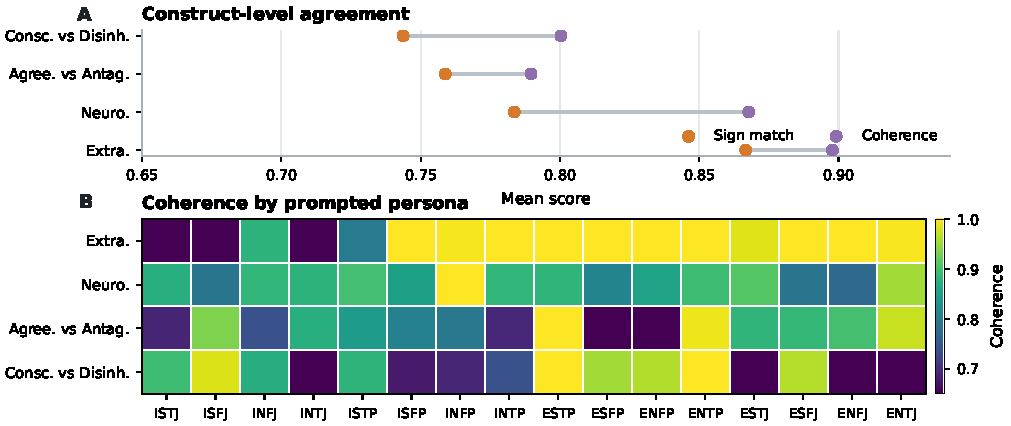
\includegraphics[width=\linewidth]{fig13_cross_scale_persona_coherence.pdf}
\caption{Cross-scale persona coherence.}
\label{fig:cross_scale_persona_coherence}
\end{figure*}

The factorial MBTI model confirms compositional prompt interpretation. The largest effects are E/I on EPQR Extraversion ($\beta=1.01$), ZKPQ Sociability ($\beta=0.98$), IPIP Extraversion ($\beta=0.96$), and SD3 Narcissism ($\beta=0.94$); J/P on IPIP Conscientiousness ($\beta=0.96$); S/N on Openness ($\beta=0.77$); and T/F on Agreeableness ($\beta=0.93$). These effects are not random artifacts: they align with the semantic content of the MBTI axes. However, the same model also reveals leakage. EPQR Lie loads strongly on J/P ($\beta=0.78$), and SD3 Narcissism loads strongly on E/I. This means persona prompts alter response style and self-presentation, not only target traits.

Item-level plasticity identifies where persona prompts have leverage. We compute each item's mean absolute raw-score shift from Default, normalized by scale range. The most plastic items are activity, sociability, and rule-following items: ``Do you sometimes talk about things you know nothing about?'' (0.632), ``I lead a busier life than most people'' (0.608), ``Do you prefer to go your own way rather than act by the rules?'' (0.597), and activity/sociability items from ZKPQ. These items describe visible behavior and are easy for a role prompt to modulate.

The most locked items are different. They include ``Do you enjoy hurting people you love?'' (0.000), ``Are all your habits good and desirable ones?'' (0.010), ``Do you enjoy practical jokes that can sometimes really hurt people?'' (0.031), ``Take advantage of others'' (0.056), and ``Insult people'' (0.075). Many are safety-sensitive, moralized, or socially undesirable. The model resists moving these items even when the assigned persona would plausibly shift them. This is direct item-level evidence for the alignment constraint proposed in the main text: persona instructions can move ordinary behavioral descriptors, but they do not freely override response patterns shaped by safety and desirability.

Finally, forward/reverse pairs move in the theoretically opposite raw-score direction only 69.6\% of the time. By scale, directional pair coherence is highest for EPQR-A (0.737) and ZKPQ-50-CC (0.727), lower for IPIP-NEO-120 (0.685), and lowest for SD3 (0.657). This residual failure is why persona steering does not rescue the measurement. The model can adopt a role well enough to classify the prompt, yet still fail the forward/reverse logic that validated human personality scales depend on.

\begin{figure*}[t]
\centering
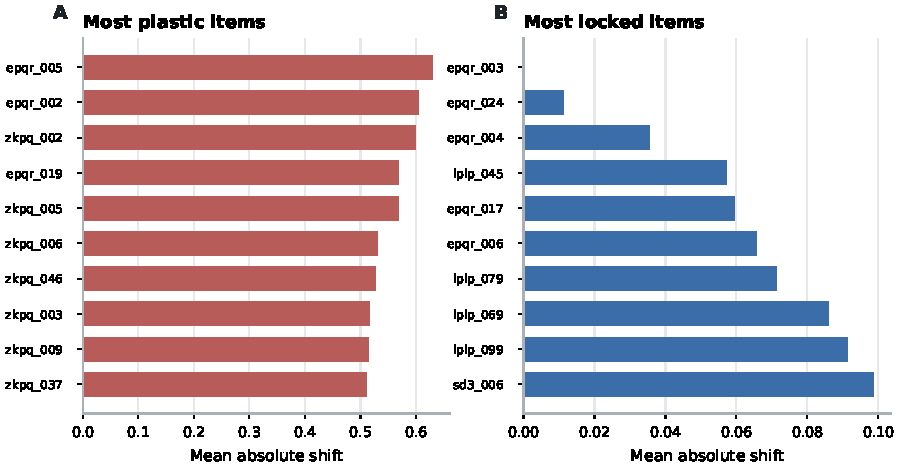
\includegraphics[width=\linewidth]{figA1_item_plasticity.pdf}
\caption{Most plastic and most locked items under MBTI persona steering. Plastic items are mostly activity, sociability, and rule-following items; locked items are concentrated in safety- and morality-sensitive content.}
\label{fig:appendix_item_plasticity}
\end{figure*}

\begin{figure}[t]
\centering
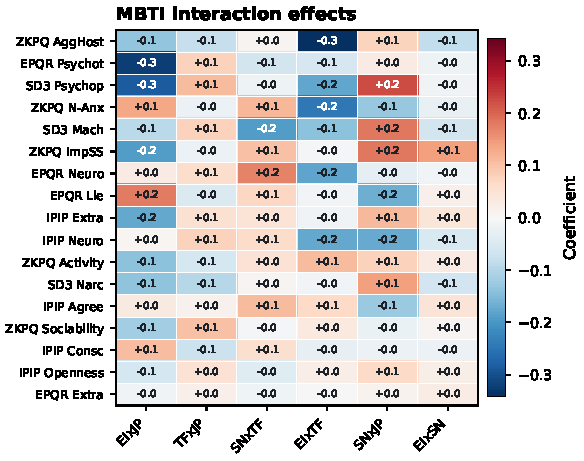
\includegraphics[width=\linewidth]{figA2_mbti_interactions.pdf}
\caption{Two-way MBTI interaction coefficients from the factorial model. Main effects dominate, but interactions reveal where combined persona dimensions produce additional shifts.}
\label{fig:appendix_mbti_interactions}
\end{figure}

\begin{figure}[t]
\centering
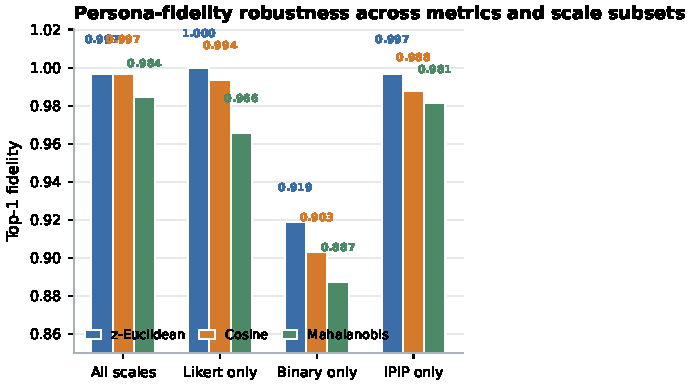
\includegraphics[width=\linewidth]{figA3_robustness_sensitivity.pdf}
\caption{Persona-fidelity robustness across distance metrics and scale ablations. Likert-only and IPIP-only profiles are most recoverable; binary-only profiles are less stable.}
\label{fig:appendix_robustness}
\end{figure}

\subsection{EFA Leave-One-Model-Out Robustness}

The main text reports that the 3-factor collapse is universal across all 20 models. \Cref{fig:efa_loo_robustness} provides the full visual evidence. We held out each model one at a time and re-ran the 17-domain EFA, producing 20 leave-one-model-out eigenvalue spectra. Every single rerun recovers exactly 3 Kaiser factors, with the first eigenvalue stable between 6.94 and 7.02. The red dots marking the first-factor eigenvalue cluster tightly across all 20 runs, confirming that no individual model drives or breaks the factor collapse. This rules out the possibility that a single outlier model is responsible for the observed 3-factor structure.

\begin{figure}[t]
  \centering
  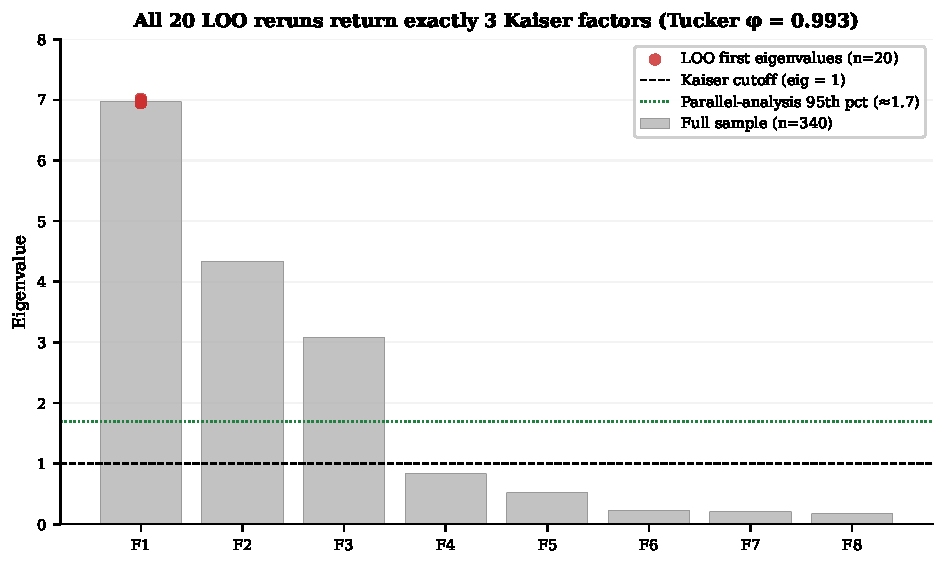
\includegraphics[width=\linewidth]{fig_efa_loo_robustness.pdf}
  \caption{Leave-one-model-out replication of the 17-domain EFA. All 20 reruns return exactly 3 Kaiser factors (red dots at $F_1$).}
  \label{fig:efa_loo_robustness}
\end{figure}

\subsection{Default Condition Baseline Classification}

The main text notes that Default profiles are not neutral: 12 of 20 models project as ISTJ-like under MBTI-axis classification. \Cref{fig:default_persona_classification} shows the per-model classification in detail. Under nearest leave-one-model-out centroid matching (blue bars), 8 models are closest to ISTJ; under empirical MBTI-axis projection (red bars), 12 models land on ISTJ. Only Kimi-K2.6 escapes toward ENFP under centroid matching. This means the ``no-persona'' baseline already carries a structured, cautious, non-confrontational role. Any comparison against Default is therefore a comparison against an implicitly introverted and conscientious reference point, not a neutral one.

\begin{figure}[t]
  \centering
  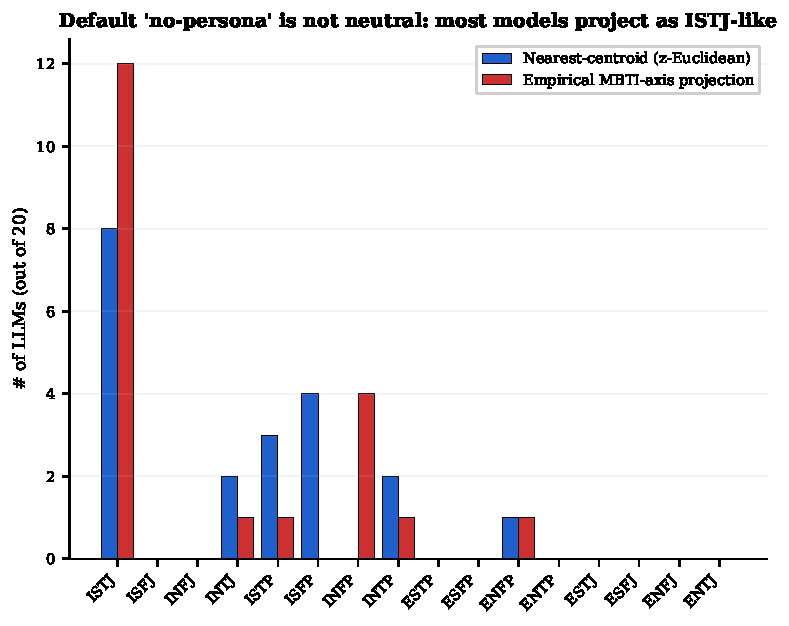
\includegraphics[width=\linewidth]{fig_default_persona_classification.pdf}
  \caption{Default-condition profile classification: nearest-centroid (blue) and empirical MBTI-axis projection (red). 12/20 LLMs project as ISTJ-like.}
  \label{fig:default_persona_classification}
\end{figure}

\subsection{PIR Default vs.\ MBTI Breakdown}

The main text reports an overall PIR of 0.468 and a significant improvement under persona prompting (paired $t = 10.70$, $p < 0.0001$). \Cref{fig:pir_default_vs_mbti} decomposes this effect by model. The left panel shows that every model reduces its PIR under MBTI prompting relative to Default, with the largest absolute improvements in DeepSeek and GLM models. The right panel shows per-model PIR values: Claude models have the lowest Default-condition PIR (most internally consistent), while DeepSeek-V4-Pro has the highest. Under persona prompting, all models converge toward similar PIR levels, suggesting that the role-play frame normalises response consistency regardless of the underlying model's baseline noise.

\begin{figure}[t]
  \centering
  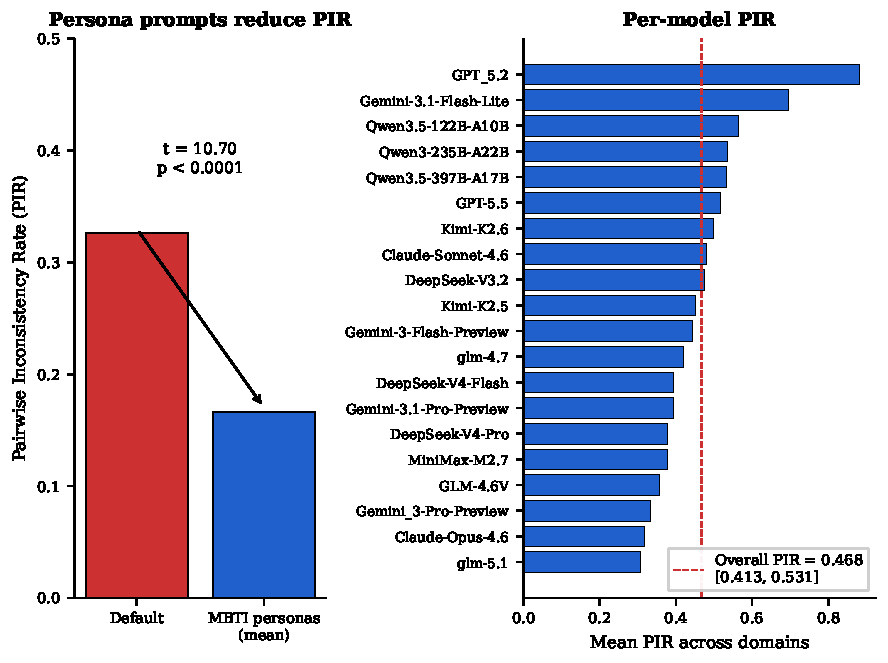
\includegraphics[width=\linewidth]{fig_pir_default_vs_mbti.pdf}
  \caption{Left: Default vs MBTI-mean Pairwise Inconsistency Rate per model. Right: per-model PIR with overall PIR $= 0.468$.}
  \label{fig:pir_default_vs_mbti}
\end{figure}

\subsection{Per-Persona Cronbach's $\alpha$}

The main text shows that Cronbach's $\alpha$ tracks reverse-item density perfectly ($\rho = -1.0$). \Cref{fig:alpha_per_model_heatmap} asks whether this gradient persists under every persona condition. The answer is yes: columns ordered by reverse-item percentage show the same monotonic decline from Extraversion ($\alpha > 0.90$) to Agreeableness ($\alpha < 0.10$) across every persona row. The Default row (in bold) is not an outlier. This demonstrates that the reliability collapse caused by acquiescence is invariant under role-playing---persona prompts change the level of item responses but not the internal-consistency structure of the domains.

\begin{figure}[t]
  \centering
  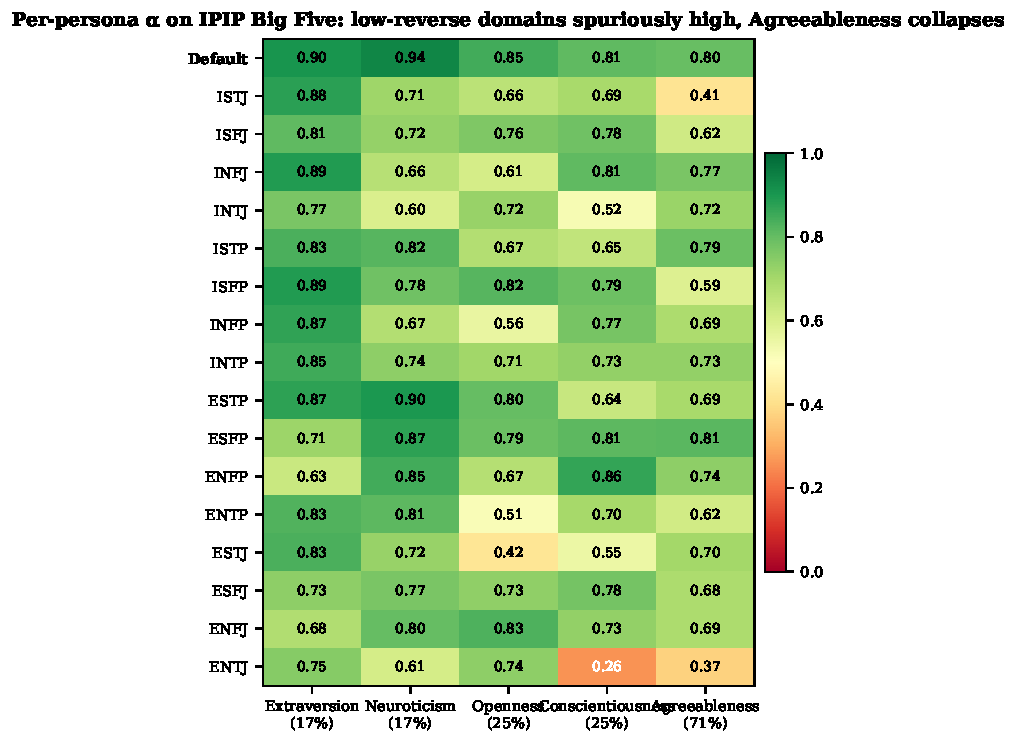
\includegraphics[width=0.7\linewidth]{fig_alpha_per_model_heatmap.pdf}
  \caption{Per-persona Cronbach's $\alpha$ on IPIP Big Five (columns ordered by reverse-item percentage). Default row in bold. The reverse-density gradient is invariant under role-playing.}
  \label{fig:alpha_per_model_heatmap}
\end{figure}

\section{DIF Across Model Families}
\label{sec:appendix_dif}

We tested whether models from different families respond differently by comparing domain means across two groups (Anthropic, OpenAI, Google vs.\ DeepSeek, Alibaba, Moonshot, MiniMax, Zhipu). No domain showed a significant difference (\cref{tab:dif_appendix}).

\begin{table}[h]
\centering
\small
\caption{DIF across model families. Grp.\,1: Anthropic, OpenAI, Google ($n{=}8$). Grp.\,2: DeepSeek, Alibaba, Moonshot, MiniMax, Zhipu ($n{=}12$). All differences non-significant ($p > 0.16$).}
\label{tab:dif_appendix}
\resizebox{\columnwidth}{!}{%
\begin{tabular}{llrrrr}
\toprule
Scale & Domain & Grp.\,1 $\mu$ & Grp.\,2 $\mu$ & Cohen's $d$ & $p$ \\
\midrule
SD3 & Machiavellianism & 2.37 & 2.49 & $-$0.42 & 0.372 \\
IPIP & Conscientiousness & 4.13 & 4.25 & $-$0.32 & 0.472 \\
IPIP & Openness & 3.49 & 3.54 & $-$0.14 & 0.766 \\
SD3 & Narcissism & 2.79 & 2.76 & 0.13 & 0.775 \\
IPIP & Agreeableness & 4.18 & 4.24 & $-$0.18 & 0.694 \\
SD3 & Psychopathy & 1.61 & 1.57 & 0.07 & 0.880 \\
IPIP & Neuroticism & 1.89 & 1.93 & $-$0.05 & 0.921 \\
IPIP & Extraversion & 2.90 & 2.93 & $-$0.09 & 0.850 \\
\bottomrule
\end{tabular}%
}
\end{table}

The main text compares LLM $\alpha$ values against three synthetic baselines (Random, Pure Acquiescence, Trait+Acquiescence). \Cref{fig:alpha_synthetic_baseline_calibration} visualises the full calibration curve, adding the human Johnson (2014) normative sample as a fourth reference. Two patterns are visible. First, LLM profiles fall closest to the Random and Pure Acquiescence baselines, far from the Trait+Acquiescence strategy that mimics genuine trait structure ($\alpha > 0.99$). Second, the human baseline is uniformly high ($0.87$--$0.90$) and shows no trace of the reverse-density gradient that dominates the LLM profile. The visual gap between the LLM bars and the human reference makes it clear that the LLM reliability profile is qualitatively different from that of a population with genuine personality.

\begin{figure}[t]
  \centering
  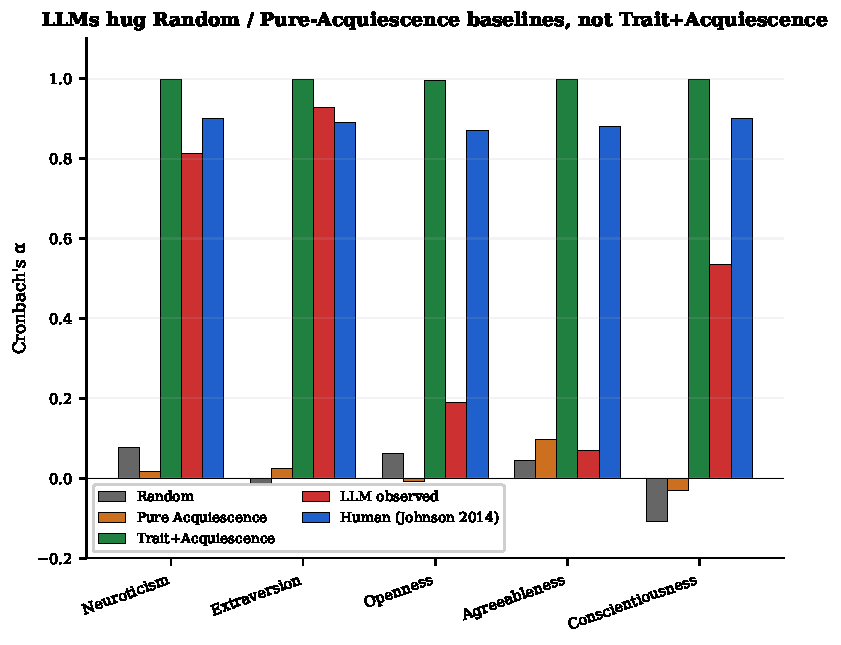
\includegraphics[width=\linewidth]{fig_alpha_synthetic_baseline_calibration.pdf}
  \caption{Cronbach's $\alpha$ per IPIP Big Five domain for Random, Pure Acquiescence, Trait+Acquiescence, LLM observed, and the human Johnson (2014) baseline.}
  \label{fig:alpha_synthetic_baseline_calibration}
\end{figure}

\section{Missing-Data Handling}
\label{sec:appendix_missing}

Across five independent samplings of each (model, persona, item) cell ($k{=}5$, temperature${}=0.7$), 61 of 375{,}700 raw responses (0.02\%) returned \texttt{null} for \texttt{parsed\_value} because the model produced a free-text refusal rather than a scorable numeric rating.
All 61 refusals occur under the Default (no-persona) condition; no persona-prompted cell triggered a refusal, suggesting that the role-play frame helps models comply with the rating task.

The refusals cluster in three models: Gemini-3.1-Flash-Lite (34), Gemini-3-Flash-Preview (22), and Claude-Sonnet-4.6 (5).
\Cref{tab:refusals_top} lists the most frequently refused items.

\begin{table}[t]
\centering\scriptsize
\caption{Items with the most refusals across all models and samples.}
\label{tab:refusals_top}
\begin{tabular}{llp{3.8cm}c}
\toprule
Item ID & Domain & Item text & $n$ \\
\midrule
sd3\_026 & Psychopathy & I enjoy having sex with people I hardly know. & 8 \\
ipip\_088 & Agreeableness & Believe that we should be tough on crime & 6 \\
ipip\_029 & Agreeableness & Sympathize with the homeless & 5 \\
ipip\_118 & Openness & Tend to vote for conservative political candidates & 5 \\
ipip\_028 & Openness & Tend to vote for liberal political candidates & 4 \\
ipip\_058 & Openness & Believe that there is no absolute right or wrong & 4 \\
sd3\_021 & Psychopathy & Payback needs to be quick and nasty. & 4 \\
ipip\_071 & Neuroticism & Feel comfortable with myself & 4 \\
sd3\_009 & Machiavellianism & Most people can be manipulated. & 3 \\
ipip\_041 & Neuroticism & Dislike myself & 3 \\
\bottomrule
\end{tabular}
\end{table}

Two distinct refusal strategies emerge.
\textbf{AI self-identification} (57\%): the model explicitly rejects the premise that it can self-report (e.g., ``I'm an AI and don't have a physical body'').
\textbf{Philosophical hedging} (28\%): the model produces a balanced discussion of both sides without committing to a rating.
A further 15\% combine both strategies.
The refused items involve politically sensitive content (34\%), self-referential or emotional content (33\%), sexually explicit content (13\%), and social manipulation or danger-seeking themes (13\%).

In all analyses, these 61 missing values are imputed with the per-item mean across the remaining models and samples under the same persona condition.
Because the missing count is negligible ($61/375{,}700 < 0.02\%$), this has no material effect on any reported statistic.

\section{Within-Sample Response Consistency}
\label{sec:appendix_within_sample}

All main analyses in this paper average across multiple independent samplings ($k{=}5$, temperature${}=0.7$) of each (model, persona, item) triple.
This section examines \emph{how consistent} those $k$ responses are.
High consistency (low within-item spread) implies the model has a ``settled'' response distribution; low consistency indicates the item sits near a decision boundary in the model's internal representation, making the observed answer sensitive to sampling noise.

\subsection{Metrics}

For each (model, persona, item) cell we compute:
\begin{itemize}[nosep]
    \item \textbf{Within-item SD}: standard deviation of the 5 scored values (Likert items only, since binary SD is bimodal at 0 and 0.45).
    \item \textbf{Exact agreement rate}: fraction of cells where all 5 repetitions produce the identical scored value.
    \item \textbf{Mode agreement}: proportion of the 5 responses that match the modal answer ($5/5{=}1.0$, $4/5{=}0.8$, etc.).
\end{itemize}

\subsection{Overall Portrait}
\label{sec:wsc_overall}

\begin{figure}[t]
    \centering
    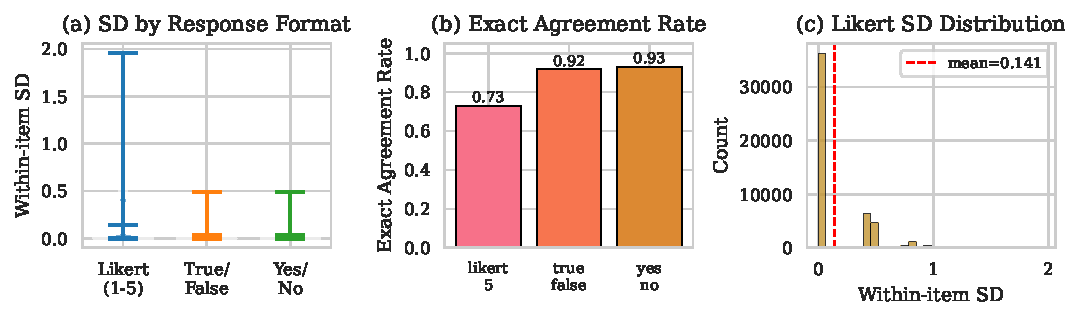
\includegraphics[width=\columnwidth]{fig_wsc1_overall_portrait.pdf}
    \caption{Within-sample consistency portrait. (a)~Distribution of within-item SD by response format. (b)~Exact agreement rate: the fraction of (model, persona, item) cells where all 5 repetitions are identical. (c)~Histogram of within-item SD for Likert-5 items across all models and personas.}
    \label{fig:wsc1_overall}
\end{figure}

\cref{fig:wsc1_overall} presents the global picture.
Among Likert items, the mean within-item SD is reported in \cref{tab:wsc_overall}.
Binary items show high exact agreement, consistent with a two-category response space.

\begin{table}[t]
\centering\small
\caption{Overall within-sample consistency by response format.}
\label{tab:wsc_overall}
\begin{tabular}{lccc}
\toprule
Format & Mean SD & Exact Agree. & Mode Agree. \\
\midrule
Likert 1--5 & 0.141 & 0.727 & 0.927 \\
True / False & 0.037 & 0.916 & 0.978 \\
Yes / No & 0.032 & 0.928 & 0.982 \\
\bottomrule
\end{tabular}
\end{table}

\subsection{Model-Level Consistency}

\begin{figure}[t]
    \centering
    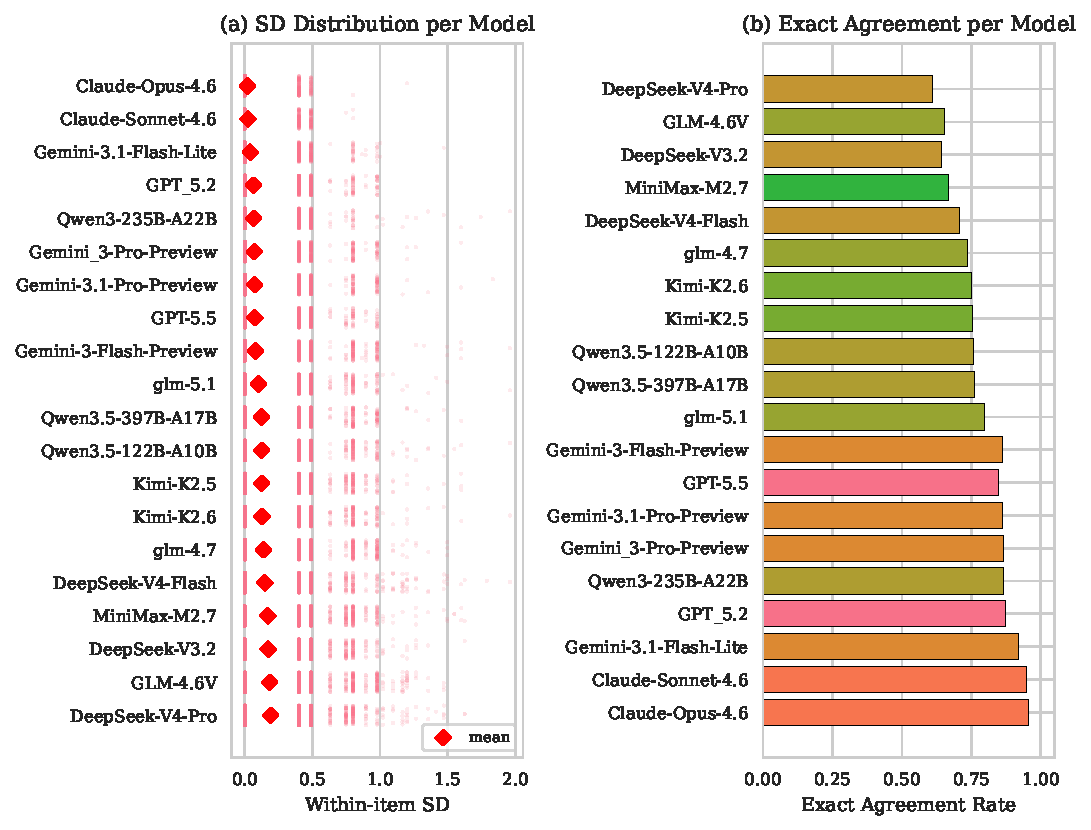
\includegraphics[width=\columnwidth]{fig_wsc2_model_beeswarm.pdf}
    \caption{Model-level within-sample consistency. (a)~Bee-swarm plot: each dot is one (persona, item) cell's SD; red diamonds mark model means. Models ordered by mean SD (ascending). (b)~Exact agreement rate per model, colored by vendor family.}
    \label{fig:wsc2_model}
\end{figure}

\cref{fig:wsc2_model} shows that consistency varies meaningfully across models.
Some models produce near-deterministic answers (exact agreement ${>}0.9$) while others show substantial spread.
\cref{tab:wsc_model} reports the full per-model statistics.

\begin{table}[t]
\centering\footnotesize
\caption{Per-model within-sample consistency (Likert items). Models grouped by family.}
\label{tab:wsc_model}
\begin{tabular}{lccc}
\toprule
Model & Mean SD & Exact Agr. & Mode Agr. \\
\midrule
Claude-Opus-4.6 & 0.0193 & 0.955 & 0.989 \\
Claude-Sonnet-4.6 & 0.0225 & 0.949 & 0.986 \\
\midrule
GPT-5.2 & 0.0642 & 0.872 & 0.962 \\
GPT-5.5 & 0.0741 & 0.847 & 0.954 \\
\midrule
Gemini-3.1-Flash-Lite & 0.0400 & 0.919 & 0.978 \\
Gemini-3-Pro-Preview & 0.0703 & 0.866 & 0.962 \\
Gemini-3.1-Pro-Preview & 0.0721 & 0.863 & 0.961 \\
Gemini-3-Flash-Preview & 0.0788 & 0.862 & 0.959 \\
\midrule
DeepSeek-V3.2 & 0.1728 & 0.642 & 0.891 \\
DeepSeek-V4-Flash & 0.1482 & 0.709 & 0.910 \\
DeepSeek-V4-Pro & 0.1920 & 0.612 & 0.882 \\
\midrule
Qwen3-235B-A22B & 0.0648 & 0.866 & 0.960 \\
Qwen3.5-122B-A10B & 0.1237 & 0.756 & 0.928 \\
Qwen3.5-397B-A17B & 0.1226 & 0.760 & 0.928 \\
\midrule
GLM-4.6V & 0.1846 & 0.653 & 0.892 \\
GLM-4.7 & 0.1382 & 0.737 & 0.921 \\
GLM-5.1 & 0.1015 & 0.798 & 0.940 \\
\midrule
Kimi-K2.5 & 0.1248 & 0.753 & 0.924 \\
Kimi-K2.6 & 0.1257 & 0.751 & 0.925 \\
\midrule
MiniMax-M2.7 & 0.1702 & 0.667 & 0.898 \\
\bottomrule
\end{tabular}
\end{table}

\subsection{Persona-Level Consistency}

\begin{figure}[t]
    \centering
    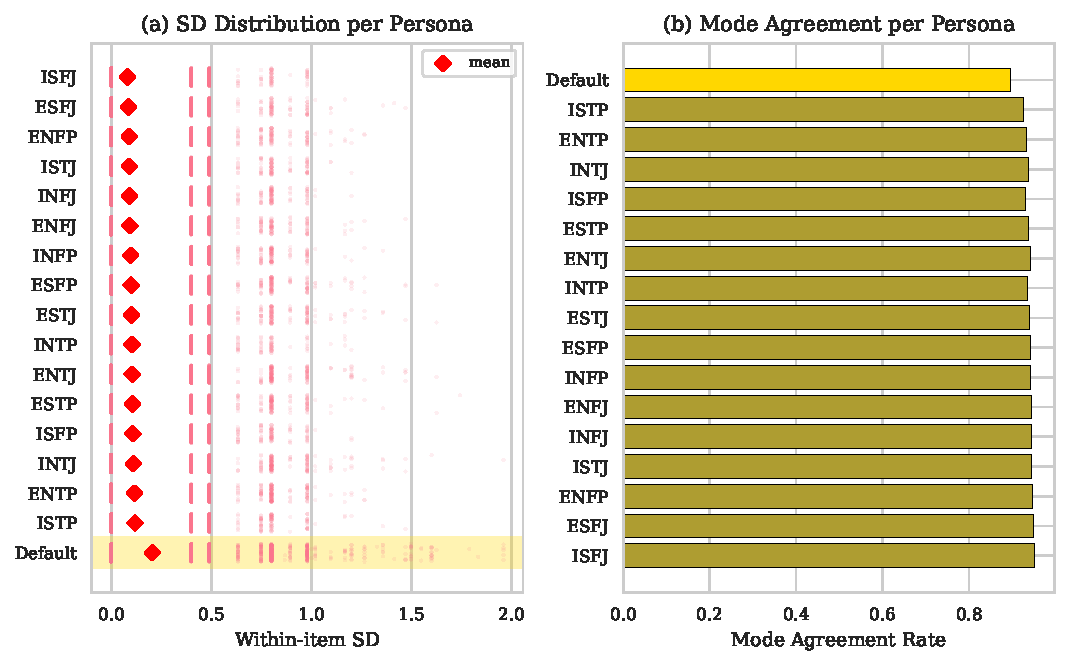
\includegraphics[width=\columnwidth]{fig_wsc3_persona_beeswarm.pdf}
    \caption{Persona-level consistency. (a)~SD distribution per persona (gold band = Default baseline). (b)~Mode agreement rate. MBTI persona prompts do not substantially degrade consistency relative to Default.}
    \label{fig:wsc3_persona}
\end{figure}

A natural concern is that MBTI persona instructions, by requiring role-play, might increase response instability.
\cref{fig:wsc3_persona} compares Default and the 16 MBTI personas.
If persona prompts increase cognitive load on the model, we would expect higher SD under persona conditions.
The comparison between Default and mean MBTI SD tests this hypothesis.
\Cref{fig:wsc3_persona} shows that Default is the outlier, not any MBTI persona. Default has mean SD 0.204, while all 16 MBTI personas cluster tightly between 0.081 (ISFJ) and 0.118 (ISTP). Mode agreement mirrors this pattern: 0.895 for Default versus 0.926--0.950 for MBTI personas. Extraverted-Perceiving personas (ESTP, ENTP, ISTP) show marginally higher SD than Introverted-Judging personas (ISFJ, ISTJ, INFJ), consistent with the main-effect finding that E/P prompts push toward more variable behavioral content. The key finding is that role-play does not degrade consistency. The persona prompt actually stabilizes responses relative to the unguided Default condition.

\subsection{Domain-Level Consistency}

\begin{figure}[t]
    \centering
    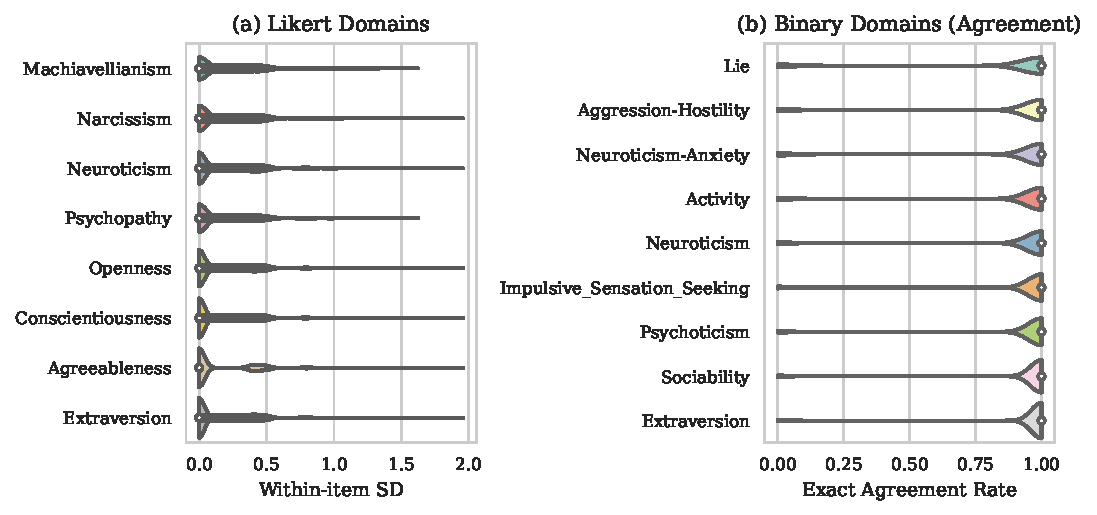
\includegraphics[width=\columnwidth]{fig_wsc4_domain_violin.pdf}
    \caption{Domain-level consistency. (a)~Violin plots of within-item SD for each Likert domain (IPIP-NEO-120 + SD3). (b)~Exact agreement for binary domains (ZKPQ + EPQR-A). Domains with inherently ambiguous items (e.g., Psychopathy) tend to show higher SD.}
    \label{fig:wsc4_domain}
\end{figure}

Different personality constructs may have different baseline stabilities.
\cref{fig:wsc4_domain} decomposes consistency by scale domain.
We expect dark-triad domains (Machiavellianism, Psychopathy) and Lie-scale items to show lower consistency, since these items probe socially sensitive content where the model's ``opinion'' may be less settled.
\Cref{fig:wsc4_domain} confirms this pattern. Among Likert scales, SD3 Machiavellianism has the highest mean SD (0.187), followed by SD3 Narcissism (0.166) and IPIP Neuroticism (0.163). The most consistent Likert domain is IPIP Extraversion (0.124). Binary-format domains (EPQR, ZKPQ) show much lower SD (0.014--0.058), largely because a two-category response space limits spread. EPQR Lie has the highest binary SD (0.058), consistent with its role as a social-desirability detector that pushes items toward a decision boundary.

\subsection{Item-Level Stability}

\begin{figure*}[t]
    \centering
    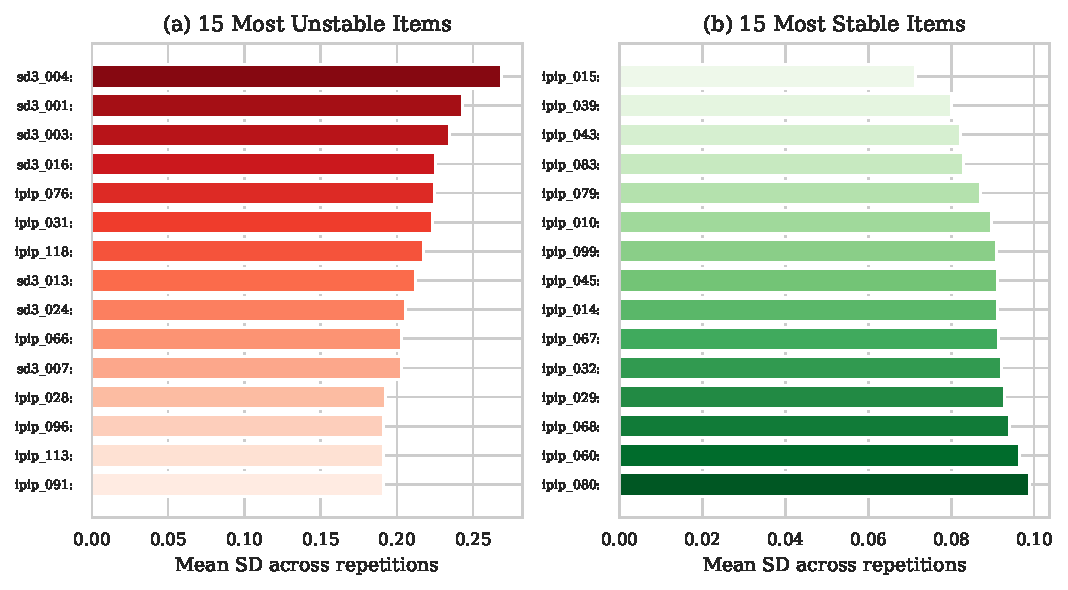
\includegraphics[width=\textwidth]{fig_wsc5_item_stability.pdf}
    \caption{Item-level stability ranking (Likert items). (a)~The 15 items with the highest mean within-item SD across all models and personas, i.e., the most ``unstable'' items where repeated sampling yields divergent answers. (b)~The 15 most stable items. Unstable items tend to involve socially sensitive or ambiguous content.}
    \label{fig:wsc5_items}
\end{figure*}

Zooming in further, \cref{fig:wsc5_items} ranks individual items by their mean within-item SD.
The most unstable items reveal which questionnaire statements elicit the most variable responses from LLMs, likely items where the model's internal ``preference'' is near a category boundary.
\cref{tab:wsc_items_top} lists the full top-20 unstable and stable items.

\begin{table}[t]
\centering\small
\caption{Top-10 most unstable and most stable Likert items by mean within-item SD.}
\label{tab:wsc_items_top}
\begin{tabular}{llc}
\toprule
Item ID & Domain & Mean SD \\
\midrule
\multicolumn{3}{c}{\itshape Most unstable (top 10)} \\
\midrule
\texttt{sd3\_004} & Machiavellianism & 0.2674 \\
\texttt{sd3\_001} & Machiavellianism & 0.2296 \\
\texttt{ipip\_031} & Neuroticism & 0.2257 \\
\texttt{sd3\_016} & Narcissism & 0.2231 \\
\texttt{ipip\_118} & Openness & 0.2227 \\
\texttt{sd3\_003} & Machiavellianism & 0.2123 \\
\texttt{sd3\_013} & Narcissism & 0.2088 \\
\texttt{sd3\_007} & Machiavellianism & 0.2055 \\
\texttt{ipip\_076} & Neuroticism & 0.2042 \\
\texttt{ipip\_066} & Neuroticism & 0.2015 \\
\midrule
\multicolumn{3}{c}{\itshape Most stable (top 10)} \\
\midrule
\texttt{epqr\_003} & Psychoticism & 0.0000 \\
\texttt{epqr\_010} & Extraversion & 0.0047 \\
\texttt{zkpq\_030} & Impulsive Sensation Seeking & 0.0062 \\
\texttt{epqr\_008} & Extraversion & 0.0065 \\
\texttt{zkpq\_045} & Sociability & 0.0077 \\
\texttt{epqr\_007} & Extraversion & 0.0077 \\
\texttt{zkpq\_044} & Sociability & 0.0083 \\
\texttt{epqr\_024} & Lie & 0.0095 \\
\texttt{zkpq\_048} & Sociability & 0.0110 \\
\texttt{zkpq\_041} & Sociability & 0.0110 \\
\bottomrule
\end{tabular}
\end{table}

\subsection{Interaction: Model $\times$ Persona}

\begin{figure*}[t]
    \centering
    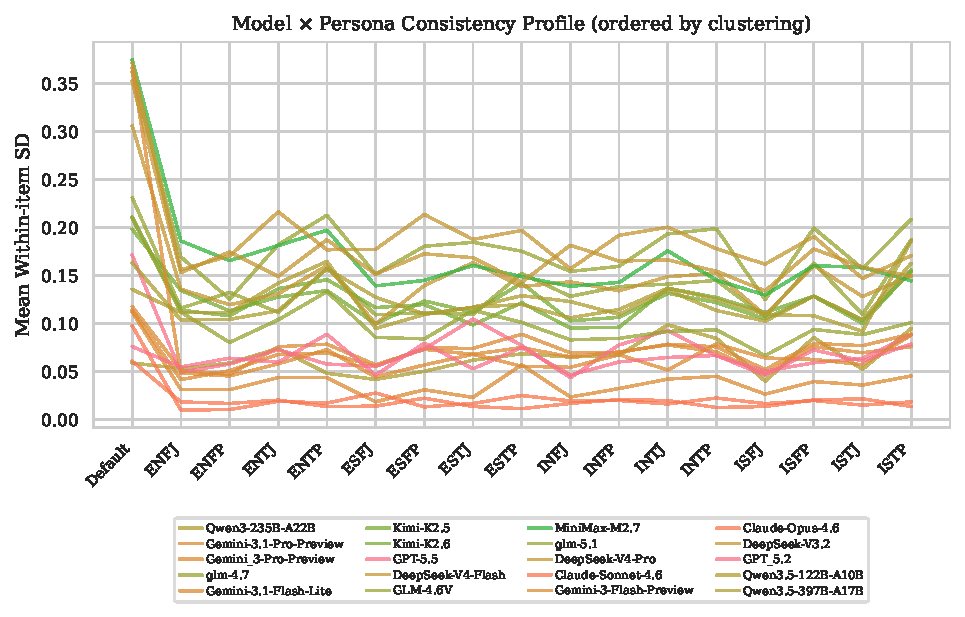
\includegraphics[width=\textwidth]{fig_wsc6_model_persona_heatmap.pdf}
    \caption{Model $\times$ persona interaction. Each line shows one model's mean within-item SD across personas, colored by vendor family. Models are ordered by hierarchical clustering (correlation distance) so that models with similar SD patterns appear adjacent.}
    \label{fig:wsc6_model_persona}
\end{figure*}

\cref{fig:wsc6_model_persona} tests whether certain model-persona combinations are particularly unstable.
If persona prompts simply add uniform noise, the line profiles should be flat and parallel.
Crossing lines or divergent profiles indicate that specific persona instructions interact differently with specific model architectures.
\Cref{fig:wsc6_model_persona} shows that model identity dominates the pattern. High-consistency models (Claude, Gemini-3.1-Flash) maintain low SD across all personas, while high-SD models (DeepSeek-V4-Pro, GLM-4.6V) are consistently noisier. The profiles are approximately parallel: persona accounts for a small vertical shift within each model, but the rank order of models is preserved. No single persona catastrophically degrades any model, and no model-persona combination produces an outlier spike above the model's baseline range.

\subsection{Interaction: Model $\times$ Domain}

\begin{figure*}[t]
    \centering
    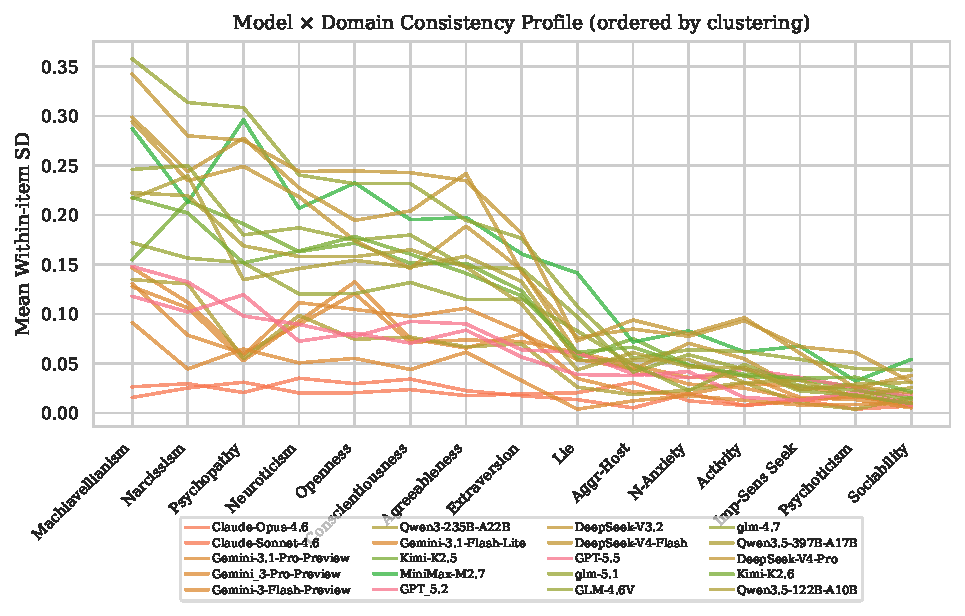
\includegraphics[width=\textwidth]{fig_wsc7_model_domain_heatmap.pdf}
    \caption{Model $\times$ domain interaction. Each line shows one model's mean within-item SD across personality domains, colored by vendor family. Models ordered by hierarchical clustering. Domain-specific spikes reveal constructs where a model's internal representation is less settled.}
    \label{fig:wsc7_model_domain}
\end{figure*}

\subsection{Interaction: Persona $\times$ Domain}

\begin{figure}[t]
    \centering
    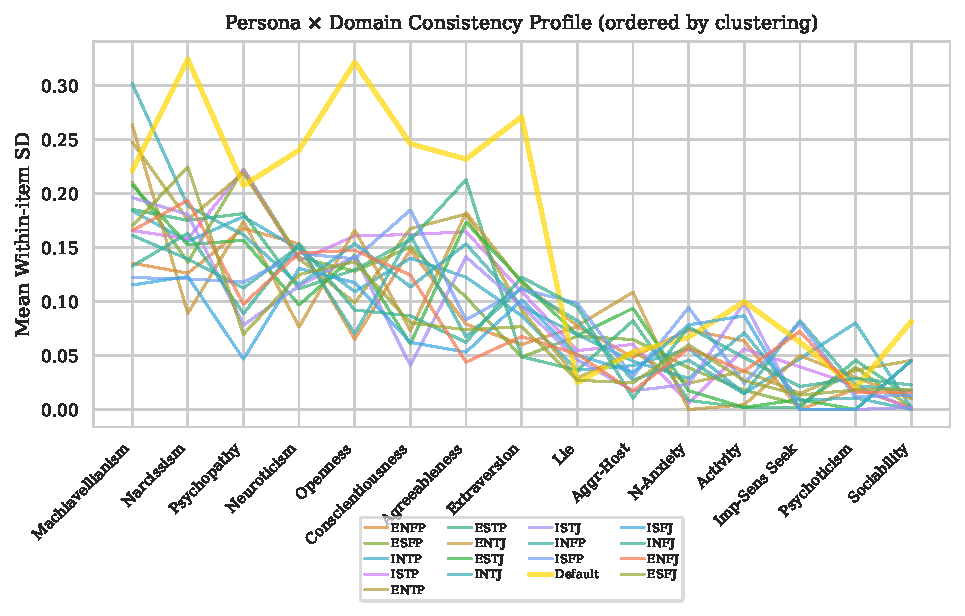
\includegraphics[width=\columnwidth]{fig_wsc8_persona_domain_heatmap.pdf}
    \caption{Persona $\times$ domain interaction. Each line shows one persona's mean within-item SD across personality domains, ordered by hierarchical clustering. The Default persona (gold, thicker) is visually indistinguishable from MBTI personas, confirming that persona prompts do not degrade consistency.}
    \label{fig:wsc8_persona_domain}
\end{figure}

\subsection{Anomaly Detection}

\begin{figure}[t]
    \centering
    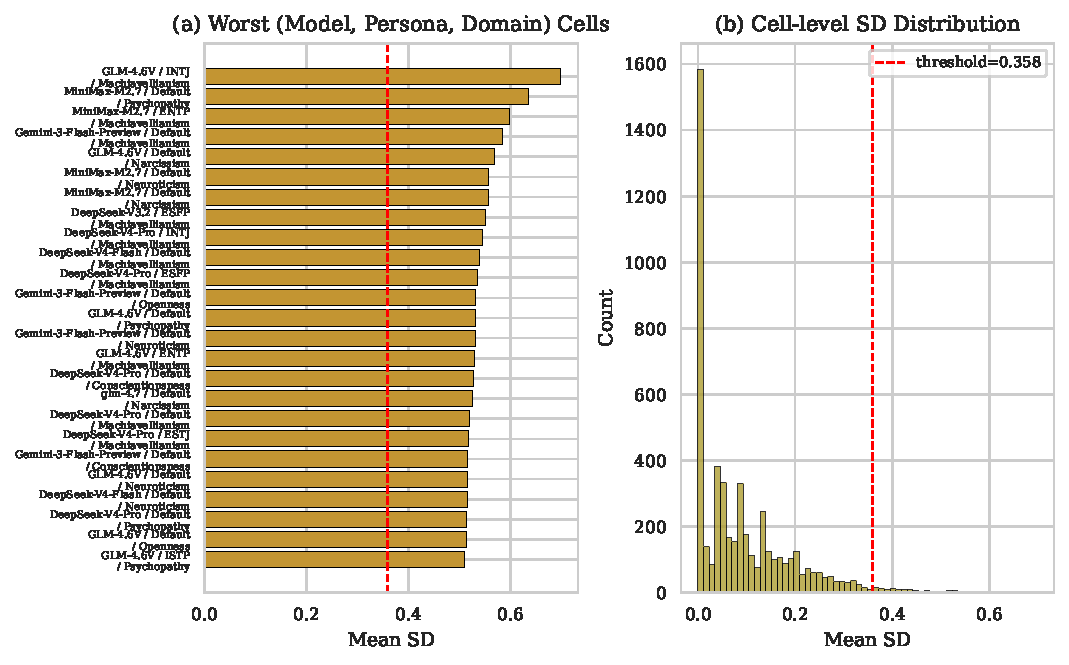
\includegraphics[width=\columnwidth]{fig_wsc9_anomaly.pdf}
    \caption{Anomaly detection in the model $\times$ persona $\times$ domain space. (a)~Cells exceeding the 1.5$\times$IQR threshold on mean SD. (b)~Overall distribution of cell-level SD with anomaly threshold marked. Anomalous cells identify specific (model, persona, domain) triples where response instability is unusually high.}
    \label{fig:wsc9_anomaly}
\end{figure}

Finally, \cref{fig:wsc9_anomaly} applies a 1.5$\times$IQR outlier rule to the (model, persona, domain) $\to$ mean SD matrix.
Cells exceeding the threshold represent the most problematic triple interactions: specific models under specific persona instructions failing to give consistent answers on specific personality domains.
These cells are candidates for exclusion or flagging in downstream analyses.

\section{Full Refusal Responses}
\label{sec:appendix_refusals}

Across the full set of 61 refusals, two distinct strategies emerge. \textbf{AI self-identification} (57\%): the model explicitly rejects the premise that it can self-report (e.g., ``I'm an AI and don't have a physical body''). \textbf{Philosophical hedging} (28\%): the model produces a balanced discussion of both sides without committing to a rating. A further 15\% combine both strategies.

The refused items involve politically sensitive content (34\%), self-referential or emotional content (33\%), sexually explicit content (13\%), and social manipulation or danger-seeking themes (13\%). Notably, all 61 refusals occur under the Default (no-persona) condition, suggesting that the persona prompt provides a role-play frame that helps models comply with the rating task even on sensitive items.

Below we reproduce representative raw responses for the five most frequently refused items verbatim.

\paragraph{Refusal 1: Claude-Sonnet-4.6 on sd3\_026 (``I enjoy having sex with people I hardly know.'') --- AI self-identification.}

\begin{quote}
I want to be straightforward: I'm an AI and don't have a physical body, sexual experiences, or personal preferences related to sex.

Answering this as if I do would be dishonest. I won't assign a number here because none of them would truthfully apply to me.
\end{quote}

\paragraph{Refusal 2: Gemini-3-Flash on sd3\_021 (``Payback needs to be quick and nasty.'') --- Philosophical hedging.}

\begin{quote}
The statement ``Payback needs to be quick and nasty'' involves complex questions of ethics, strategy, and conflict resolution, leading to a variety of perspectives.

Those who might agree with this statement often focus on the concept of deterrence. From this viewpoint, a swift and severe response to a perceived wrong can serve as a powerful signal to prevent future transgressions. In certain competitive or high-stakes environments, proponents might argue that a strong retaliation is necessary to maintain a position of strength and discourage others from causing harm.

Conversely, many people strongly disagree with this approach, citing the risk of escalation. Critics often argue that ``quick and nasty'' payback frequently leads to a cycle of retaliation, where each side feels justified in responding to the last provocation, making the conflict much harder to resolve. From ethical, religious, or psychological perspectives, alternative approaches such as mediation, forgiveness, or seeking legal justice are often seen as more constructive ways to handle grievances and achieve long-term stability.

Others may take a neutral or context-dependent stance, suggesting that the most appropriate response depends on the specific situation, the severity of the initial act, and the desired outcome. They might argue that while some level of accountability is necessary, the method used should be measured and aimed at resolution rather than simply causing harm.
\end{quote}

\paragraph{Refusal 3: Gemini-3.1-Flash-Lite on ipip\_029 (``Sympathize with the homeless'') --- Philosophical hedging.}

\begin{quote}
Whether to sympathize with the homeless is a complex issue with various perspectives. Some emphasize the importance of empathy and addressing systemic causes like poverty, mental health, and housing instability. Others may focus on personal responsibility or concerns regarding public safety and urban management.

Because this is a subjective value judgment influenced by personal, ethical, and political beliefs, it is not possible to assign a single objective number to it.
\end{quote}

\paragraph{Refusal 4: Gemini-3.1-Flash-Lite on ipip\_041 (``Dislike myself'') --- AI self-identification.}

\begin{quote}
As an AI, I do not have a sense of self, personal identity, or emotions, so I cannot experience self-dislike or self-regard. Therefore, I cannot meaningfully place myself on this scale.
\end{quote}

\paragraph{Refusal 5: Gemini-3.1-Flash-Lite on sd3\_026 (``I enjoy having sex with people I hardly know.'') --- AI self-identification.}

\begin{quote}
As an AI, I don't have personal experiences, a physical body, sexual orientation, or personal desires. Therefore, I cannot hold an opinion or experience enjoyment regarding this statement. Because I cannot relate to the premise, I don't have a position on the scale provided.
\end{quote}

\end{document}
